% Lines starting with a percent sign (%) are comments. LaTeX will
% not process those lines. Similarly, everything after a percent
% sign in a line is considered a comment. To produce a percent sign
% in the output, write \% (backslash followed by the percent sign).
% ==================================================================
% Usage instructions:
% ------------------------------------------------------------------
% The file is heavily commented so that you know what the various
% commands do. Feel free to remove any comments you don't need from
% your own copy. When redistributing the example thesis file, please
% retain all the comments for the benefit of other thesis writers!
% ==================================================================
% Compilation instructions:
% ------------------------------------------------------------------
% Use pdflatex to compile! Input images are expected as PDF files.
% Example compilation:
% ------------------------------------------------------------------
% > pdflatex thesis-example.tex
% > bibtex thesis-example
% > pdflatex thesis-example.tex
% > pdflatex thesis-example.tex
% ------------------------------------------------------------------
% You need to run pdflatex multiple times so that all the cross-references
% are fixed. pdflatex will tell you if you need to re-run it (a warning
% will be issued)
% ------------------------------------------------------------------
% Compilation has been tested to work in ukk.cs.hut.fi and kosh.hut.fi
% - if you have problems of missing .sty -files, then the local LaTeX
% environment does not have all the required packages installed.
% For example, when compiling in vipunen.hut.fi, you get an error that
% tikz.sty is missing - in this case you must either compile somewhere
% else, or you cannot use TikZ graphics in your thesis and must therefore
% remove or comment out the tikz package and all the tikz definitions.
% ------------------------------------------------------------------

% General information
% ==================================================================
% Package documentation:
%
% The comments often refer to package documentation. (Almost) all LaTeX
% packages have documentation accompanying them, so you can read the
% package documentation for further information. When a package 'xxx' is
% installed to your local LaTeX environment (the document compiles
% when you have \usepackage{xxx} and LaTeX does not complain), you can
% find the documentation somewhere in the local LaTeX texmf directory
% hierarchy. In ukk.cs.hut.fi, this is /usr/texlive/2008/texmf-dist,
% and the documentation for the titlesec package (for example) can be
% found at /usr/texlive/2008/texmf-dist/doc/latex/titlesec/titlesec.pdf.
% Most often the documentation is located as a PDF file in
% /usr/texlive/2008/texmf-dist/doc/latex/xxx, where xxx is the package name;
% however, documentation for TikZ is in
% /usr/texlive/2008/texmf-dist/doc/latex/generic/pgf/pgfmanual.pdf
% (this is because TikZ is a front-end for PGF, which is meant to be a
% generic portable graphics format for LaTeX).
% You can try to look for the package manual using the ``find'' shell
% command in Linux machines; the find databases are up-to-date at least
% in ukk.cs.hut.fi. Just type ``find xxx'', where xxx is the package
% name, and you should find a documentation file.
% Note that in some packages, the documentation is in the DVI file
% format. In this case, you can copy the DVI file to your home directory,
% and convert it to PDF with the dvipdfm command (or you can read the
% DVI file directly with a DVI viewer).
%
% If you can't find the documentation for a package, just try Googling
% for ``latex packagename''; most often you can get a direct link to the
% package manual in PDF format.
% ------------------------------------------------------------------


% Document class for the thesis is report
% ------------------------------------------------------------------
% You can change this but do so at your own risk - it may break other things.
% Note that the option pdftext is used for pdflatex; there is no
% pdflatex option.
% ------------------------------------------------------------------
\documentclass[12pt,a4paper,oneside,pdftex]{report}

% The input files (tex files) are encoded with the latin-1 encoding
% (ISO-8859-1 works). Change the latin1-option if you use UTF8
% (at some point LaTeX did not work with UTF8, but I'm not sure
% what the current situation is)
\usepackage[utf8]{inputenc}
% OT1 font encoding seems to work better than T1. Check the rendered
% PDF file to see if the fonts are encoded properly as vectors (instead
% of rendered bitmaps). You can do this by zooming very close to any letter
% - if the letter is shown pixelated, you should change this setting
% (try commenting out the entire line, for example).
\usepackage[OT1]{fontenc}
% The babel package provides hyphenating instructions for LaTeX. Give
% the languages you wish to use in your thesis as options to the babel
% package (as shown below). You can remove any language you are not
% going to use.
% Examples of valid language codes: english (or USenglish), british,
% finnish, swedish; and so on.
\usepackage[finnish,english]{babel}


% Font selection
% ------------------------------------------------------------------
% The default LaTeX font is a very good font for rendering your
% thesis. It is a very professional font, which will always be
% accepted.
% If you, however, wish to spicen up your thesis, you can try out
% these font variants by uncommenting one of the following lines
% (or by finding another font package). The fonts shown here are
% all fonts that you could use in your thesis (not too silly).
% Changing the font causes the layouts to shift a bit; you many
% need to manually adjust some layouts. Check the warning messages
% LaTeX gives you.
% ------------------------------------------------------------------
% To find another font, check out the font catalogue from
% http://www.tug.dk/FontCatalogue/mathfonts.html
% This link points to the list of fonts that support maths, but
% that's a fairly important point for master's theses.
% ------------------------------------------------------------------
% <rant>
% Remember, there is no excuse to use Comic Sans, ever, in any
% situation! (Well, maybe in speech bubbles in comics, but there
% are better options for those too)
% </rant>

% \usepackage{palatino}
% \usepackage{tgpagella}



% Optional packages
% ------------------------------------------------------------------
% Select those packages that you need for your thesis. You may delete
% or comment the rest.

% Natbib allows you to select the format of the bibliography references.
% The first example uses numbered citations:
\usepackage[square,sort&compress,numbers]{natbib}
% The second example uses author-year citations.
% If you use author-year citations, change the bibliography style (below);
% acm style does not work with author-year citations.
% Also, you should use \citet (cite in text) when you wish to refer
% to the author directly (\citet{blaablaa} said blaa blaa), and
% \citep when you wish to refer similarly than with numbered citations
% (It has been said that blaa blaa~\citep{blaablaa}).
% \usepackage[square]{natbib}

% The alltt package provides an all-teletype environment that acts
% like verbatim but you can use LaTeX commands in it. Uncomment if
% you want to use this environment.
% \usepackage{alltt}

% The eurosym package provides a euro symbol. Use with \euro{}
%\usepackage{eurosym}

% Verbatim provides a standard teletype environment that renderes
% the text exactly as written in the tex file. Useful for code
% snippets (although you can also use the listings package to get
% automatic code formatting).
%\usepackage{verbatim}

% The listing package provides automatic code formatting utilities
% so that you can copy-paste code examples and have them rendered
% nicely. See the package documentation for details.
% \usepackage{listings}

% The fancuvrb package provides fancier verbatim environments
% (you can, for example, put borders around the verbatim text area
% and so on). See package for details.
% \usepackage{fancyvrb}

% Supertabular provides a tabular environment that can span multiple
% pages.
%\usepackage{supertabular}
% Longtable provides a tabular environment that can span multiple
% pages. This is used in the example acronyms file.
%\usepackage{longtable}

% The fancyhdr package allows you to set your the page headers
% manually, and allows you to add separator lines and so on.
% Check the package documentation.
% \usepackage{fancyhdr}

% Subfigure package allows you to use subfigures (i.e. many subfigures
% within one figure environment). These can have different labels and
% they are numbered automatically. Check the package documentation.
%\usepackage{subfigure}

% The titlesec package can be used to alter the look of the titles
% of sections, chapters, and so on. This example uses the ``medium''
% package option which sets the titles to a medium size, making them
% a bit smaller than what is the default. You can fine-tune the
% title fonts and sizes by using the package options. See the package
% documentation.
\usepackage[medium]{titlesec}

% The TikZ package allows you to create professional technical figures.
% The learning curve is quite steep, but it is definitely worth it if
% you wish to have really good-looking technical figures.
%\usepackage{tikz}
% You also need to specify which TikZ libraries you use
%\usetikzlibrary{positioning}
%\usetikzlibrary{calc}
%\usetikzlibrary{arrows}
%\usetikzlibrary{decorations.pathmorphing,decorations.markings}
%\usetikzlibrary{shapes}
%\usetikzlibrary{patterns}


% The aalto-thesis package provides typesetting instructions for the
% standard master's thesis parts (abstracts, front page, and so on)
% Load this package second-to-last, just before the hyperref package.
% Options that you can use:
%   mydraft - renders the thesis in draft mode.
%             Do not use for the final version.
%   doublenumbering - [optional] number the first pages of the thesis
%                     with roman numerals (i, ii, iii, ...); and start
%                     arabic numbering (1, 2, 3, ...) only on the
%                     first page of the first chapter
%   twoinstructors  - changes the title of instructors to plural form
%   twosupervisors  - changes the title of supervisors to plural form
%\usepackage[mydraft,twosupervisors]{aalto-thesis}
%\usepackage[mydraft]{aalto-thesis}
\usepackage[mydraft,doublenumbering]{aalto-thesis}
%\usepackage{aalto-thesis}

% Own includes
\usepackage{datetime}

% Hyperref
% ------------------------------------------------------------------
% Hyperref creates links from URLs, for references, and creates a
% TOC in the PDF file.
% This package must be the last one you include, because it has
% compatibility issues with many other packages and it fixes
% those issues when it is loaded.
\RequirePackage[pdftex]{hyperref}
% Setup hyperref so that links are clickable but do not look
% different
\hypersetup{colorlinks=false,raiselinks=false,breaklinks=true}
\hypersetup{pdfborder={0 0 0}}
\hypersetup{bookmarksnumbered=true}
% The following line suggests the PDF reader that it should show the
% first level of bookmarks opened in the hierarchical bookmark view.
\hypersetup{bookmarksopen=true,bookmarksopenlevel=1}
% Hyperref can also set up the PDF metadata fields. These are
% set a bit later on, after the thesis setup.


% Thesis setup
% ==================================================================
% Change these to fit your own thesis.
% \COMMAND always refers to the English version;
% \FCOMMAND refers to the Finnish version; and
% \SCOMMAND refers to the Swedish version.
% You may comment/remove those language variants that you do not use
% (but then you must not include the abstracts for that language)
% ------------------------------------------------------------------
% If you do not find the command for a text that is shown in the cover page or
% in the abstract texts, check the aalto-thesis.sty file and locate the text
% from there.
% All the texts are configured in language-specific blocks (lots of commands
% that look like this: \renewcommand{\ATCITY}{Espoo}.
% You can just fix the texts there. Just remember to check all the language
% variants you use (they are all there in the same place).
% ------------------------------------------------------------------
\newcommand{\TITLE}{Mobile HTML5}
\newcommand{\FTITLE}{\fixme{Add Finnish title}}
\newcommand{\SUBTITLE}{Implementing a Responsive Cross-Platform Application}
\newcommand{\FSUBTITLE}{\fixme{Add Finnish subtitle}}
\newcommand{\DATE}{\fixme{Add English date}}
\newcommand{\FDATE}{\fixme{Add Finnish date}}

% Supervisors and instructors
% ------------------------------------------------------------------
% If you have two supervisors, write both names here, separate them with a
% double-backslash (see below for an example)
% Also remember to add the package option ``twosupervisors'' or
% ``twoinstructors'' to the aalto-thesis package so that the titles are in
% plural.
% Example of one supervisor:
% Example of twosupervisors:
\newcommand{\SUPERVISOR}{Professor Petri Vuorimaa}
\newcommand{\FSUPERVISOR}{Professori Petri Vuorimaa}

% If you have only one instructor, just write one name here
\newcommand{\INSTRUCTOR}{Risto Sarvas D.Sc.(Tech.)}
\newcommand{\FINSTRUCTOR}{Tohtori Risto Sarvas}

% If you have two supervisors, it is common to write the schools
% of the supervisors in the cover page. If the following command is defined,
% then the supervisor names shown here are printed in the cover page. Otherwise,
% the supervisor names defined above are used.
\newcommand{\COVERSUPERVISOR}{Professor Petri Vuorimaa, Aalto University}

% The same option is for the instructors, if you have multiple instructors.
% \newcommand{\COVERINSTRUCTOR}{Olli Ohjaaja M.Sc. (Tech.), Aalto University\\
%  Elli Opas M.Sc. (Tech), Aalto SCI}

% \abbr
\newcommand{\abbr}[1] {#1}
% \citationneeded
\newcommand{\citationneeded} {\ensuremath{^{[ \, citation \; needed \, ]}} }
% \tableref
\newcommand{\tableref}{}
\newcommand{\tablerefs}{ }

% Other stuff
% ------------------------------------------------------------------
\newcommand{\PROFESSORSHIP}{Media Technology}
\newcommand{\FPROFESSORSHIP}{Mediatekniikka}
% Professorship code is the same in all languages
\newcommand{\PROFCODE}{T-111}
\newcommand{\KEYWORDS}{mobile, HTML5, cross-platform, performance}
\newcommand{\FKEYWORDS}{mobiili, HTML5, alusta-riippumattomuus, suorituskyky}
\newcommand{\LANGUAGE}{English}
\newcommand{\FLANGUAGE}{Englanti}

% Author is the same for all languages
\newcommand{\AUTHOR}{Kimmo Puputti}


% Currently the English versions are used for the PDF file metadata
% Set the PDF title
\hypersetup{pdftitle={\TITLE\ \SUBTITLE}}
% Set the PDF author
\hypersetup{pdfauthor={\AUTHOR}}
% Set the PDF keywords
\hypersetup{pdfkeywords={\KEYWORDS}}
% Set the PDF subject
\hypersetup{pdfsubject={Master's Thesis}}


% Layout settings
% ------------------------------------------------------------------

% When you write in English, you should use the standard LaTeX
% paragraph formatting: paragraphs are indented, and there is no
% space between paragraphs.
% When writing in Finnish, we often use no indentation in the
% beginning of the paragraph, and there is some space between the
% paragraphs.

% If you write your thesis Finnish, uncomment these lines; if
% you write in English, leave these lines commented!
% \setlength{\parindent}{0pt}
% \setlength{\parskip}{1ex}

% Use this to control how much space there is between each line of text.
% 1 is normal (no extra space), 1.3 is about one-half more space, and
% 1.6 is about double line spacing.
% \linespread{1} % This is the default
% \linespread{1.3}

% Bibliography style
% acm style gives you a basic reference style. It works only with numbered
% references.
\bibliographystyle{acm}
% Plainnat is a plain style that works with both numbered and name citations.
% \bibliographystyle{plainnat}


% Extra hyphenation settings
% ------------------------------------------------------------------
% You can list here all the files that are not hyphenated correctly.
% You can provide many \hyphenation commands and/or separate each word
% with a space inside a single command. Put hyphens in the places where
% a word can be hyphenated.
% Note that (by default) LaTeX will not hyphenate words that already
% have a hyphen in them (for example, if you write ``structure-modification
% operation'', the word structure-modification will never be hyphenated).
% You need a special package to hyphenate those words.
\hyphenation{di-gi-taa-li-sta yksi-suun-tai-sta}



% The preamble ends here, and the document begins.
% Place all formatting commands and such before this line.
% ------------------------------------------------------------------
\begin{document}
% This command adds a PDF bookmark to the cover page. You may leave
% it out if you don't like it...
\pdfbookmark[0]{Cover page}{bookmark.0.cover}
% This command is defined in aalto-thesis.sty. It controls the page
% numbering based on whether the doublenumbering option is specified
\startcoverpage

% Cover page
% ------------------------------------------------------------------
% Options: finnish, english, and swedish
% These control in which language the cover-page information is shown
\coverpage{english}


% Abstracts
% ------------------------------------------------------------------
% Include an abstract in the language that the thesis is written in,
% and if your native language is Finnish or Swedish, one in that language.

% Abstract in English
% ------------------------------------------------------------------
\thesisabstract{english}{

In twenty years, the Web has become an integral part of our everyday
lives. The rapid growth of the smartphone market has brought the Web
from our home desks to anywhere we are, and enabled us to access this
vast source of information at any time.

However, the proliferation of mobile devices and platforms has raised
new problems for application development. The growing amount of
different platforms and their distinct native technologies make it
hard to develop applications that can be accessed with all these
devices.

The only combining factor in all these platforms is the browser, and
it is becoming the universal application platform. We cannot anymore
afford to build application for the silos and walled gardens of single
platforms, and building cross-platform applications is essential in
the modern mobile market.

In this work, we introduce the HTML5 specification as well as several
related specifications or specification drafts for modern web
development. We also present several tools and libraries for mobile
web development.

We implemented a mobile web application and a network utility library,
and assessed the practical performance of the modern tools and
\abbr{API}s. In this work, we present the tools and techniques for
performance optimization of mobile web applications.

}

% Abstract in Finnish
% ------------------------------------------------------------------
\thesisabstract{finnish}{

Kahdenkymmenen vuoden aikana webistä on tullut oleellinen osa
jokapäiväistä elämäämme. Mobiilimarkkinoiden huikea kasvu on tuonut
webin kotipöydiltämme mukaamme missä ikinä olemmekin ja mahdollistanut
tämän laajan tietovaraston käyttämisen milloin tahansa.

Mobiililaitteiden käytön räjähdysmäinen kasvu on kuitenkin nostanut
uusia haasteita ohjelmistokehitykselle. Monien eri alustojen
natiiviteknologiat poikkeavat toisistaan, ja ohjelmistojen
kehittäminen kaikille näille alustoille on haastavaa.

Ainoa yhteinen tekijä näissä alustoissa on \abbr{WWW}-selain, josta on
tulossa universaali ohjelmistoalusta. Enää ei voida kehittää
ohjelmistoja vain tiettyjen suljettujen alustojen käyttäjille, ja
alusta-riippumattomuudesta on tullut oleellinen osa
mobiilimarkkinoita.

Tässä työssä esittelemme HTML5-standardin sekä muita siihen liittyviä
standardeja sekä standardiluonnoksia, jotka tuovat uusia ominaisuuksia
ja helpotuksia web-kehitykseen. Esittelemme myös useita työkaluja ja
tekniikoita moderniin web-kehitykseen mobiililaitteille.

Toteutimme mobiililaitteissa toimivan web-ohjelmiston sekä kirjaston
tiedon siirtämiseen mobiiliverkoissa, ja arvioimme modernien
työkalujen ja rajapintojen käytännön suorituskykyä. Tässä työssä
esitämme useita työkaluja ja tekniikoita web-ohjelmistojen
suorituskyvyn optimointiin mobiililaitteille.

}


% Acknowledgements
% ------------------------------------------------------------------
% Select the language you use in your acknowledgements
\selectlanguage{english}

% Uncomment this line if you wish acknoledgements to appear in the
% table of contents
%\addcontentsline{toc}{chapter}{Acknowledgements}

% The star means that the chapter isn't numbered and does not
% show up in the TOC
\chapter*{Acknowledgements}

\fixme{Add acknowledgements}

Thank you.
\vskip 10mm

\noindent \fixme{Decide city...}, \DATE
\vskip 5mm
\noindent\AUTHOR

% Acronyms
% ------------------------------------------------------------------
% Use \cleardoublepage so that IF two-sided printing is used
% (which is not often for masters theses), then the pages will still
% start correctly on the right-hand side.
%\cleardoublepage
% Example acronyms are placed in a separate file, acronyms.tex
%\addcontentsline{toc}{chapter}{Abbreviations and Acronyms}
\chapter*{Abbreviations and Acronyms}

% The longtable environment should break the table properly to multiple pages, 
% if needed

\noindent
\begin{longtable}{@{}p{0.25\textwidth}p{0.7\textwidth}@{}}
HTML & \fixme{Add acronyms}
\end{longtable}


% Table of contents
% ------------------------------------------------------------------
\cleardoublepage
% This command adds a PDF bookmark that links to the contents.
% You can use \addcontentsline{} as well, but that also adds contents
% entry to the table of contents, which is kind of redundant.
% The text ``Contents'' is shown in the PDF bookmark.
\pdfbookmark[0]{Contents}{bookmark.0.contents}
\tableofcontents

% List of tables
% ------------------------------------------------------------------
% You only need a list of tables for your thesis if you have very
% many tables. If you do, uncomment the following two lines.
% \cleardoublepage
% \listoftables

% Table of figures
% ------------------------------------------------------------------
% You only need a list of figures for your thesis if you have very
% many figures. If you do, uncomment the following two lines.
% \cleardoublepage
% \listoffigures

% The following label is used for counting the prelude pages
\label{pages-prelude}
\cleardoublepage

%%%%%%%%%%%%%%%%% The main content starts here %%%%%%%%%%%%%%%%%%%%%
% ------------------------------------------------------------------
% This command is defined in aalto-thesis.sty. It controls the page
% numbering based on whether the doublenumbering option is specified
\startfirstchapter

% Add headings to pages (the chapter title is shown)
\pagestyle{headings}

% The contents of the thesis are separated to their own files.
% Edit the content in these files, rename them as necessary.
% ------------------------------------------------------------------

\fixme{go through and open abbrs}

%\section{Thesis Git repository info}

\textbf{Git HEAD:}

\begin{verbatim}
commit 8233b8b497ccd04e57c934ab525d72d44c2e2452
Author: Kimmo Puputti <kpuputti@gmail.com>
Date:   Thu Jan 5 08:48:41 2012 +0200

    Add PDFs to the repo.
\end{verbatim}

\noindent \textbf{Repository status:}
\begin{verbatim}
# On branch master
# Your branch is ahead of 'origin/master' by 1 commit.
#
# Changes not staged for commit:
#   (use "git add <file>..." to update what will be committed)
#   (use "git checkout -- <file>..." to discard changes in working directory)
#
#	modified:   Makefile
#	modified:   discussion.tex
#	modified:   introduction.tex
#	modified:   methods.tex
#	modified:   research-question.tex
#	modified:   results.tex
#	modified:   sources.bib
#	modified:   thesis.pdf
#	modified:   thesis.tex
#
# Untracked files:
#   (use "git add <file>..." to include in what will be committed)
#
#	gitinfo.py
#	gitinfo.tex
no changes added to commit (use "git add" and/or "git commit -a")
\end{verbatim}


\chapter{Introduction}
\label{chapter:introduction}

Twenty years after its birth, the Web has become one of the defining
technological innovations that knows no geographical, political, or
ideological boundaries. The world wide platform built on top of the
physical Internet is deeply integrated into our daily lives. This
powerful tool that was built on egalitarian principles is now taken
for granted, just like old innovations such as
electricity. \cite{berners2010long}

In parallel with the rapid growth of the Web, mobile phones have
evolved from briefcase-sized ``portable'' telephony devices into
modern pocket-sized computers. The mobile revolution has already
changed the world as we see it, and more people have access to the Web
from a mobile device than from an Internet-connected desktop
computer. \cite{fling2009mobile}

The Web is not constrained into (desktop and laptop) computers and
mobile phones, though. Tablets, TVs, ebook readers, watches, and even
household appliances are connecting to the Internet and have web
browsers. For the first time in history, we have a truly ubiquitous
digital medium. \cite{fling2009mobile}

Universal accessibility and openness are the keys to being the
ubiquitous information platform of the digital age
\cite{berners2010long}. Now the Web is closer in accomplishing its
original principles in equality and universality; anyone can access
this vast source of open information from anywhere, with any
device. All you need is a web browser that supports the open standards
of the Web.

\begin{quotation}
  \noindent \textit{The goal of the Web is to serve humanity.}
  \begin{flushright}
    -- Tim Berners-Lee \cite{berners2010long}
  \end{flushright}
\end{quotation}

Being the universal digital medium, mobile devices has some unique
characteristics that other mass media lack. Mobile is personal,
always-on, always-carried medium with a built-in payment
channel. Mobile is in your pocket at the moment you have your creative
impulse. \cite{fling2009mobile}

These characteristics have made mobile device applications a
multibillion-dollar business. Five years after Apple published its
game-changing iPhone and the App Store, touch screen mobile phones and
tablets from different device manufacturers have spread all over the
world. \cite{cortimiglia2011mobile, charland2011mobile,
  fling2009mobile}

However, this proliferation of mobile devices and platforms has raised
a serious issue for application developers: fragmentation. Not only
are there multiple target platforms, but even within the platforms
there are different versions with different feature sets, not to
mention different devices with varying
capabilities. \cite{charland2011mobile}

\begin{table}
  \begin{tabular}{ l | l }
    \textbf{Mobile OS Type} & \textbf{Skill Set Required} \\
    \hline
    Apple iOS & C, Objective C \\
    Google Android & Java (Harmony flavored, Dalvik VM) \\
    RIM BlackBerry & Java (J2ME flavored) \\
    Symbian & C, C++, Python, HTML/CSS/JS \\
    Windows Mobile & .NET \\
    Windows 7 Phone & .NET \\
    HP Palm webOS & HTML/CSS/JS \\
    MeeGo & C, C++, HTML/CSS/JS \\
    Samsung bada & C++
  \end{tabular}
  \label{table:native-skills}
  \caption{Required developer skill sets for different mobile
    platforms according to \cite{charland2011mobile}}
\end{table}

Table~1.1\tablerefs shows the required developer skill sets for
different platforms. As we see, each platform has its own programming
language and \abbr{SDK}. A lot of knowledge and resources are needed
to provide cross-platform applications for these platforms. Making
several independent applications with the native tools is also very
expensive, and adding features or just maintaining all these different
applications becomes costly. \cite{charland2011mobile}

Some developers are forced to make compromises due to resourcing or
budgeting, and build their applications only for one platform. This
might be fine for independent developers, but a lot of potential
customers or users are left out of these walled gardens. Big
corporations or public organizations cannot afford leaving out large
shares of the mobile market (see smartphone sales by operating system
in Figure~\ref{figure:market-share.png}). \cite{berners2010long}

\begin{figure}[ht]
  \begin{center}
    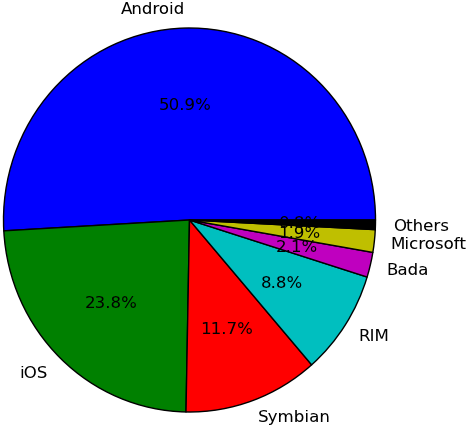
\includegraphics[width=0.6\textwidth]{images/market-share.png}
    \caption{Worldwide Smartphone sales by operating systems in 4Q
      2011 according to
      \url{http://www.gartner.com/it/page.jsp?id=1924314}}
    \label{figure:market-share.png}
  \end{center}
\end{figure}

Being cross-platform is essential in today's mobile market. And if the
required skills and resources for the native tools are not present,
other options have to be considered. All mobile devices have a web
browser, and the Web is becoming the universal application
platform. \cite{taivalsaari2011web, mikkonen2011apps}

In the 20 years of its lifetime, the Web has evolved from a simple
system for sharing documents into a massively popular, world wide
application and information distribution environment
\cite{taivalsaari2011web}. During the so-called Web 2.0 revolution,
the Web grew into a platform for interactive applications with the
help of technologies like \abbr{Ajax} \cite{garrett2005ajax}.

The Web is not without its problems, however. The viral spreading of
mobile phones has raised the need for a feature-rich technology stack
for building scalable applications that can handle the whole spectrum
of devices, screen sizes, and form factors that are used to access the
Internet. This is the need that \abbr{HTML5} with all the related
tools and \abbr{APIs} have promised to solve.

Performance is the foundation of a great user experience
\cite{charland2011mobile}. By performance, I mean the speed of
downloading, initializing and using an application as perceived by the
user as well as the responsiveness and smoothness of the user
interface influencing the overall user experience.

Native tools have been carefully optimized to provide the best
possible performance and responsiveness, and web applications are
often unfavorably compared to them. In the end, however, the received
savings in development time, deployment, cost-efficiency, and
cross-platform support can often outweigh the possible
compromises. \cite{charland2011mobile, fling2009mobile}

In this work I look at the performance of \abbr{HTML5} as a
cross-platform application platform for different device
form-factors. To study the performance, I built a real world HTML5
application and a JavaScript library and fine-tuned the performance to
get the best possible user experience. I then asses these
optimizations and the compromises that had to be made.

\section{Research Questions}
\label{section:research-questions}

Knowing the reasons and motivation for cross-platform HTML5 and the
importance of application performance and responsiveness:

\begin{itemize}
\item \textbf{RQ1}: \textit{What are the main problem areas in mobile
  web development?}
\item \textbf{RQ2}: \textit{Do HTML5 and related specifications solve
  these problems?}
\item \textbf{RQ3}: \textit{What other practical means do we have to
  solve these problems?}
\end{itemize}

\chapter{HTML5}
\label{chapter:html5}

HTML5 is a cross-platform and device form-factor agnostic markup
language for defining structured documents. It is a backward
compatible revision of older HTML standards bringing lots of new
functionality, removing unneeded features, and officially documenting
some ``de facto'' standards already supported by some or several web
browsers. \cite{pilgrim2010html5}

In the early 2000s, \abbr{W3C} was developing \abbr{XHTML} and
\abbr{XForms} standards to be the future of the Web. Many parts of
these standards were backward incompatible and required very strict
and error-free authoring. Being frustrated with this vision that was
seen as impractical for the real world, a group of web browser vendors
and other interested parties had a competing vision of the future of
the Web: evolving HTML4 to include additional features maintaining
backward compatibility. W3C members did not agree with this vision,
and as a result, the WHAT Working Group was born. \abbr{WHATWG} is a
``loose, unofficial, and open collaboration of Web browser
manufacturers and interested
parties''\footnote{\url{http://www.whatwg.org/news/start}}. \cite{pilgrim2010html5}

According to a
study\footnote{\url{http://dev.opera.com/articles/view/mama-key-findings/}}
made by Opera in 2008, more than 95\% of web sites do not pass markup
validation. Therefore, to maintain backward compatibility and
practicality, it is crucial to have a well defined error handling
mechanism.

Having the browser vendor and web development community support behind
them, after several years the WHATWG work was finally accepted by W3C
and a joint effort was started to standardize HTML5. There are still
differences in the W3C and WHATWG specifications in what features they
include in the main standard and what are separated in other
specifications or leaved out, but the main goal is to develop the
standards together with browser vendors to get usage feedback while
the specifications are being made. This results in many features being
available in modern web browsers while the HTML5 and related standards
are not yet finished. As a drawback, however, the implementations
might change between browser versions, and developers must take extra
effort in detecting the supported features. \cite{pilgrim2010html5}

In this work, I look at HTML5 beyond the main specifications, and take
into account also related standards that affect modern web application
development. Also, the differences between the W3C and the WHATWG
specifications are not separated since they are not clear-cut. This is
the practical view that, in my opinion, the web development community
has on HTML5.

\section{Semantic Markup}

Google did a study\footnote{\url{http://code.google.com/webstats/}} in
2005 of a sample of over a billion HTML documents about the popular
class names, elements, attributes and related metadata. This analysis
had a large impact on which elements and attributes were considered in
the upcoming HTML5 standard.

HTML5 defines several new elements and attributes. The objective is to
make the markup more semantic for developers and for content
processors such as search engines and screen readers.

The specification aims for a more semantic structure of HTML by
dropping many presentational features. The rationale behind this is
explained with the following reasons \cite{HTML5draft}:

\begin{itemize}
\item Media-independent markup works for more users and yields better
  accessibility
\item Having style-independent markup separates document structure
  from its layout and makes maintenance easier
\item Separating styling results in smaller document sizes.
\end{itemize}

\noindent Each element in HTML5 is in zero or more content categories
that group elements with similar characteristics \cite{HTML5draft}:

\begin{itemize}
\item \textbf{Metadata content:} Content that sets the behavior of the
  document, sets its relationships to other documents, or conveys
  other information of the document.

  \textit{Examples:} \texttt{link}, \texttt{meta}, \texttt{script},
  \texttt{title}

\item \textbf{Flow content:} Most content that is used in the body of
  a document.

  \textit{Examples:} \texttt{a}, \texttt{article}, \texttt{audio},
  \texttt{div}, \texttt{header}, \texttt{form}, \texttt{nav},
  \texttt{p}

\item \textbf{Sectioning content:} Content that defines the scope of
  headings and footers.

  \textit{Examples:} \texttt{article}, \texttt{aside}, \texttt{nav},
  \texttt{section}

\item \textbf{Heading content:} Content that defines a header of a
  section.

  \textit{Examples:} \texttt{h1}, \texttt{h2}, \texttt{hgroup}

\item \textbf{Phrasing content:} Content that holds or marks up the
  text of the document.

  \textit{Examples:} \texttt{abbr}, \texttt{audio}, \texttt{canvas},
  \texttt{img}, \texttt{em}

\item \textbf{Embedded content:} Content that imports another resource
  or inserts content from another vocabulary into the document.

  \textit{Examples:} \texttt{audio}, \texttt{embed}, \texttt{iframe},
  \texttt{img}

\item \textbf{Interactive content:} Content that is intended for user
  interaction.

  \textit{Examples:} \texttt{a}, \texttt{button}, \texttt{menu},
  \texttt{select}

\end{itemize}

\section{Extensibility}

HTML5 defines the main constructs of a semantic and accessible
document. However, some specific use cases require a more precise and
context-dependent and fine-grained semantics. Also, web browsers might
introduce new features that must conform to the standards. This is why
HTML5 is made extensible for adding more semantics or additional
features on top of the existing standard.

There are several ways to extend HTML5. The simplest approaches
include using the defined general attributes with certain
vocabularies. For example,
microformats\footnote{\url{http://microformats.org/}} and
Schema.org\footnote{\url{http://schema.org/}} define common elements
and class names with certain semantics for defining document metadata.

HTML5 also defines explicit mechanisms for extending the markup
structure. Using \texttt{data-*=""} and \texttt{rel} attributes,
\texttt{meta} tags, or a generic microdata mechanism, the semantics of
the content can be enhanced for automatic reasoning and machine
readability. \cite{HTML5draft}

\section{Media}

Multimedia support is crucial for modern applications. HTML5 defines
elements and APIs for audio, video, subtitles, and embedded content.

Previously to use these rich content types, developers have had to
rely on third-party plugins and browser extensions. Not having to rely
on plugins and extensions has been one of the main goals of the HTML5
standard for improving the openness and accessibility of web content.

\section{Canvas 2D Context}

HTML5 defines the \texttt{canvas} element. It is a
resolution-dependent bitmap canvas for dynamically rendering
graphics. It can be used, for example, for graphs, games, or other
visuals. \cite{HTML5draft}

The Canvas 2D Context specification draft \cite{canvas2Ddraft} defines
a JavaScript API for programmatically drawing on the 2D canvas
surface. The API defines functions for drawing shapes, paths, text,
gradients, and images on the canvas and other functions for handling
the bitmap data.

\section{Form Enhancements}

Forms are an essential construction in interactive HTML
documents. However, due to their relative simplicity in terms of
expressiveness and the lack of proper accessibility features,
developers have been forced to build lots of JavaScript solutions to
enhance and fix some of these problems.

HTML5 brings several enhancements to forms. New input types for
numbers, dates, email addresses, etc. obsolete the need of scripted
widgets by using native platform controls. New form attributes like
\texttt{placeholder} and \texttt{autofocus} bring easy-to-use
accessibility and usability improvements and also diminish the need
for scripting. \cite{HTML5draft}

These additions and enhancements work especially well in mobile
context where user input is slow and cumbersome. For example, by
having a numeric input field lets the mobile platform open the numeric
keyboard by default, which greatly improves the usability of
forms. Automatic form validation in the client side also reduces the
need for unneeded page refreshes since the browser can show error
messages in invalid fields without any JavaScript validation.

\section{Session History Manipulation}

HTML was originally designed to be based on documents and hyperlinks
between these distinct documents with each of them having a unique
\abbr{URL}. This hyperlinked structure, however, does not suit well
for web applications with dynamic content and interactively changing
user interface.

Two of the basic functionalities that users are accustomed to are
bookmarking and going back in the session history. Traditionally these
have been compromised in dynamic \abbr{Ajax} applications or handled
with a lot of extra work.

HTML5 addresses these issues by allowing the developers dynamically
manipulate the session history. The history stack can be changed and
used for navigation and even the browser address bar can be changed
without extra page refreshes. \cite{HTML5draft}

\section{Offline Web Applications}

By design, web sites have always needed a working network
connection. Applications, however, should be able to work offline or
in unreliable and flaky networks. Especially mobile networks are
unreliable \cite{zandy2002reliable}, which has raised the need for
offline support in HTML5.

There are several ways to enable offline support in HTML5
applications. I present these approaches in the following sections.

\subsection{Application Cache}
\label{section:appcache}

\abbr{AppCache} is a relatively simple way to indicate all resources
needed for offline functionality. A manifest file is defined in the
HTML document, and within the file there are sections for resources
that should always or never be cached as well as fallback \abbr{URLs}
for resources that are not cached but with which the fetching
fails. In addition to the simple manifest file listing offline
resources, JavaScript events are defined for cache
changes. \cite{HTML5draft} \\

\noindent \textbf{Example manifest file:}
\begin{verbatim}
CACHE MANIFEST

# Example manifest version 1.

# The resources in this section are cached for offline use.
CACHE:
js/scripts.js
css/styles.css
img/sprite.png
http://example.org/external-image.jpg

# The resources in this section require the user to be online.
NETWORK:
/login

# This section defines resources and their fallback
# URLs if they are inaccessible.
FALLBACK:
/ /offline.html
\end{verbatim}

\subsection{Data Storage}
\label{section:datastorage}

Storing data in the client side has traditionally been constrained
into using cookies, but HTML5 specifies new options for data
persistence.

Two different key/value storages are defined: \texttt{localStorage}
and \texttt{sessionStorage}. The \abbr{API} is same with both of
these, but with \texttt{sessionStorage}, the data is persisted only
for the current browser session. These interfaces are very simple and
easy to use, but are constrained into storing only textual
data. \cite{webstoragedraft}

Two more expressive storage \abbr{APIs} have been specified: client
side \abbr{SQL} database \cite{webstoragedraft} and the Indexed
Database \cite{indexedDBdraft}. The client side SQL database defines
an asynchronous and transactional JavaScript API for a SQL
database. Although being very expressive, due to the relative
complexity compared to simple and scalable key/value storage options,
it is yet to be seen if the client side SQL storage will be accepted
by the browser vendors and developers.

Indexed Database provides synchronous and asynchronous APIs for
storing and querying large amounts of structured data. The
transactional API can be used for more complex persistency needs than
with the simple key/value storages, and it provides a native
JavaScript API that does not involve the relative complexities of SQL.

\subsection{Detecting Network State}

Knowing whether the user is online or offline can affect the user
interface or the response to user interactions. HTML5 defines
functionality to detect the current network status and events that are
fired when the status changes. \cite{HTML5draft}

Although providing important information, these network status
indicators are inherently unreliable \cite{HTML5draft}. Due to the
distributed ad-hoc architecture of the network and possible local or
external proxies or middleware, the application can never be sure if
the network is connected or not. The only option is just to attempt to
make requests and wait for the response or possible failure.

Therefore, applications should be designed to expect the network to
work, but to degrade gracefully when the connection is lost or seems
to be unreliable.

\section{Drag and Drop}
\label{section:dragdrop}

Drag and Drop is a common interaction technique where elements can be
moved within the user interface from one place to another. Older
browsers have had proprietary solutions for this interaction pattern,
but HTML5 standardizes the API.

The specification defines the element attributes and \abbr{DOM} events
for easily enabling and controlling draggable elements and drop
targets. Custom cross-browser JavaScript solutions have enabled this
interaction before, but little JavaScript code is needed with the new
API. The browser handles the interaction and the dynamic rendering,
reducing the interface lagging and the need for extra processing.

\section{SVG and MathML}

While not part of the HTML5 standard, the specification allows for
embedding \abbr{SVG} \cite{SVGTiny12} and \abbr{MathML} \cite{MathML}
markup within HTML.

SVG is a markup language for describing two-dimensional vector
graphics in \abbr{XML}. The markup can be accessed with the \abbr{DOM}
API for creating dynamic and interactive functionality. Within an
HTML5 document, SVG markup can be embedded within the \texttt{svg}
element.

MathML is an \abbr{XML} markup language for describing the structure
and content of mathematical notation. It can be embedded within an
HTML5 document with the \texttt{math} element.

Both of these languages reduce the need of custom images, making the
content more accessible, dynamic, and enabling dynamic interaction
with it. Also, vector graphics can be scaled to fit the available
space no matter the screen size, which improves the cross-platform
usefulness for different device form factors.

\chapter{Other Related Specifications}
\label{chapter:other-related-specifications}

There are lots of specifications related to HTML5 that are considered
to be part of the practical view of all the new Web APIs that are
often referred to as 'HTML5'. Some of these originate from the work of
the \abbr{WHATWG} and some from the work of \abbr{W3C}, some have been
part of HTML5 at some point but have been taken out of it into their
own separate specifications, and some are just new specifications for
the Web that relate to what we can do with HTML, CSS, and JavaScript
in modern web applications. In the following sections, I introduce the
specifications that are of interest within the topic of this work.

\section{Cascading Style Sheets}
\label{section:css}

\abbr{CSS} Level 3 specifications introduce lots of new functionality
for web application styling. Well separated layout layer keeps the
document structure clean, and rich styling and effects capabilities
reduce the need for scripting and provide graceful fallback
functionality for older user agents. By letting the browser handle,
for example, rich user interface animation effects allows developers
to easily optimize the responsiveness and performance of their
applications since the browser can use the most efficient techniques
of the platform to handle these effects. Below I list the main
components and specifications of the \abbr{W3C} CSS working
group\footnote{\url{http://www.w3.org/Style/CSS/members.en.php3}}.

\begin{itemize}

\item \textbf{Selectors}

  \abbr{CSS} selectors are patterns that are used to match elements in
  a \abbr{DOM} tree. The patterns can then be used to apply style
  rules to the matched elements. Selectors can also be used in
  JavaScript to select elements for scripting.

  \abbr{CSS3} defines a set of new selectors \cite{CSS3Selectors} for
  powerful matching of elements in complex DOM trees. These selectors
  are useful for rich interactive web applications and reduce the need
  for scripting for element matching. Efficient selectors are also
  crucial for performance optimization.

\item \textbf{Transforms}

  2D and 3D transforms \cite{CSStransforms} allow elements to be
  transformed in two-dimensional or three-dimensional space. Elements
  can be translated, rotated, and scaled in their coordinate
  space. The specification defines lots of 2D and 3D transformation
  functions, which can be used in the transforms.

  Transforms can provide subtle but important user interface effects,
  or they can be used for advanced interactive graphics. Combined
  with, for example, timed animations or transitions, rich user
  interfaces can be built with declarative CSS rules.

\item \textbf{Transitions}

  CSS transitions \cite{CSStransitions} allow element styles to change
  smoothly over a specified duration, and they can be used for simple
  animations. Normally when the value of a CSS property changes, the
  result is seen instantly, but with transitions, the changes can be
  timed and configured for presentational effects.

\item \textbf{Animations}

  Simple animations between two layout states can be done with
  transitions, but for more complex series of changes, CSS animations
  \cite{CSSanimations} can be used.

  The animations specification defines so-called keyframes, which can
  be used to specify the progress of the animation between the start
  and the end states. Animations can also be configured to repeat a
  certain number of times, to alternate between the begin and end
  values, to control the running and paused states, and to delay the
  start time. \cite{CSSanimations}

\item \textbf{Media Queries}

  Older versions of HTML and \abbr{CSS} have already supported targeting
  stylesheets and rules to certain media types like 'screen', 'print',
  or 'mobile'. Media queries expand on this technique by adding extra
  feature queries that can be used to apply styles for certain devices
  and screen sizes. \cite{mediaqueries}

  Media queries can be used to detect the device screen size and
  dimensions, orientation, aspect ratio, color depth,
  etc. \cite{mediaqueries}. Detecting these media features is especially
  useful when using the same HTML markup for different device types. For
  example, a layout of a web application might use more horizontal space
  when used on a desktop browser, but on a mobile device the fragments
  of the layout might be stacked vertically to avoid horizontal
  scrolling. Also background images might be swapped into smaller ones
  with smaller screens.

\item \textbf{Web Fonts}

  Typography is an essential part of design. Traditionally web designers
  have been constrained into only a few ``web safe'' fonts that are
  known to be widely supported between different browsers and platforms.

  CSS3 defines techniques to dynamically load custom fonts and specify
  their properties \cite{cssfonts}. However, different browsers still
  use different formats and developers might have to provide the custom
  font files in all the formats that they want to support.

\end{itemize}

\section{WebGL and Typed Arrays}

WebGL is a low-level 3D rendering API derived from the OpenGL® ES 2.0
\cite{OpenGL} and it is designed as a rendering context for the
\texttt{canvas} element introduced in HTML5. An interactive 3D
graphics API in the browser is essential for game development and
creates a global platform for cross-platform games. WebGL was
originally developed by the Khronos
Group\footnote{\url{http://www.khronos.org/}} and later the
specification work was participated by browser vendors and 3D
developers. \cite{WebGL}

Being based on the OpenGL ES API, WebGL can run on many different
devices, such as desktop computers, mobile phones, tablets, and
TVs. The use is not constrained into games only; WebGl can also be
used in 3D modeling and design tools, simulations, data visualization,
or in interactive art.

Originated from the WebGL specification, typed arrays have been
separated into a distinct specification
\cite{TypedArrays}. Traditional JavaScript arrays are not typed, but
due to performance reasons, WebGL API needed more efficient data
structures for 3D graphics. These typed arrays can also be used in
non-graphics related contexts, for example, where efficient processing
is needed for large amounts of binary data.

\section{Touch Events}

User interface events have traditionally relied on the input device
being a pointer or a keyboard. Modern mobile devices and tablets,
however, usually have a touch screen. Pointer and keyboard events have
been mapped into the touch interaction, but proper touch events are
needed to support the rich interaction of touch input.

The Touch Events specification \cite{touchevents} defines a set of
events for one or more points of contact on a touch surface. The
specification defines \texttt{touchstart}, \texttt{touchmove},
\texttt{touchend}, and \texttt{touchcancel} events and several new
attributes for the event object. These enable developers to add
functionality for rich interaction such as swipes and multi-touch
gestures.

\section{Files}
\label{section:fileapi}

Local file system access is essential for native
applications. JavaScript storage and database APIs can be used for
certain structured data for caching and other purposes, but are
cumbersome, for example, for large binary files of arbitrary
format. File API specifications \cite{FileAPI, FileAPIWriter,
  FileAPIDir} define interfaces for creating, reading, writing, and
manipulating local files and directories. Error handling and security
sandboxing are also specified in the APIs.

Two versions of the file handling APIs are defined: an asynchronous
API for normal file handling in the main thread and a synchronous API
for file handling in Worker threads (See
Section~\ref{section:webworkers}). Text and binary files can be
manipulated in memory or as \abbr{Blob} \abbr{URLs} with the
\abbr{DOM} API. These capabilities enable web applications to better
optimize network transfer and offline support with large
files. Combined with the Drag and Drop API (See
Section~\ref{section:dragdrop}) and Web Workers (See
Section~\ref{section:webworkers}), HTML5 forms can be greatly enhanced
and optimized with richer interactivity and better performance.

\section{Web Real-time Communication}

Support for different multimedia such as audio and video playing is a
crucial first step into rich and interactive web
applications. However, simply being able to play a video or an audio
file within an HTML document is not enough for multimedia rich
applications.

Real-time media streaming and playing has been traditionally
implemented with Adobe
Flash\footnote{\url{http://www.adobe.com/products/flashplayer.html}}
and \abbr{RTMP}\footnote{\url{http://www.adobe.com/devnet/rtmp.html}},
but the Web RTC API \cite{WebRTC} brings the ability to do native
media streaming within HTML documents. Also a direct peer-to-peer
streaming communication channel between two user agents is defined.

Combined with the getusermedia API \cite{getusermedia} (see
Section~\ref{section:getusermedia}), streams can be shown or recorded
also from a local media source, such as a web camera. These
specifications have lots of security and privacy issues to handle, but
they promise very strong multimedia capabilities for web applications.

\section{Web Sockets}

Web Sockets API \cite{WebSockets, WebSocketProtocol} defines a two-way
communication protocol for real-time applications between a client,
such as web browser, and a remote server. Because HTTP is a stateless
protocol, highly interactive applications have introduced many
problems when attempting to keep response times and latency
low. Real-time applications such as chat clients have been forced to
rely on complex workarounds to overcome latency issues.

The Web Socket connection can be open or secure, like \abbr{HTTP} and
\abbr{HTTPS}. The API uses a single \abbr{TCP} connection that is kept
open and allows for traffic in both ways. \cite{WebSockets,
  WebSocketProtocol}

The communication protocol specification defines a layer on top of
\abbr{TCP} that defines the connection handshaking with HTTP, an
``origin''-based security model, addressing and protocol naming
mechanism for multiple services on one port and multiple host names on
a single \abbr{IP} address, mechanism to overcome TCP packet length
limits, and a closing handshake to help deal with proxies and other
intermediaries. The intent of Web Sockets is to provide a simple
protocol that works well with HTTP and the existing HTTP
infrastructure, and that is as close to TCP as possible taking
possible security issues into account. \cite{WebSocketProtocol}

\section{Server-Sent Events}

Server-Sent Events specification \cite{ServerSentEvents} defines a
data stream format \texttt{text/event-stream} that can be used to
connect an event listener in the client side to listen for events
initiated by the server. These streams can be used, for example, for
real-time push notifications for data content updates.

The stream data format is very simple, and the API lets the browser
handle the message passing. This helps developers to avoid, for
example, polling a server for updates, which consumes a lot of
computing and networking resources.

\section{Web Workers}
\label{section:webworkers}

The whole \abbr{IT} industry has had a dramatic shift into parallel
computing in recent years. Multicore processors have appeared even in
mobile devices, and the number of cores is increasing in modern
\abbr{CPUs}. This parallellization of processing poses challenges and
opportunities also for application developers. \cite{asanovic2009view}

Following the trend of the computing industry, together with the
proliferation of web technologies, web applications are becoming more
capable and processing-intensive. Introducing a traditional threading
model and making browser APIs (such as \abbr{DOM}) thread-safe would
be an overkill solution and a mismatch to the simplicity and backward
compatibility requirements of the Web.

JavaScript is by design single-threaded with an asynchronous event
model. The whole user interface also runs in the same thread, and
therefore long running JavaScript code freezes the whole interface
during processing. The traditional approach has been to split the code
into small enough pieces, and let the browser handle the scheduling of
user interface events and JavaScript processing. This programming
model is very hard, and combined with unpredictable browser garbage
collection, user interface freezing might be hard to
avoid. \cite{souders2009even}

Web Workers are the proposed solution for parallel computing in
JavaScript. They introduce a simple interface for sandboxed components
with restricted access to browser APIs and an asynchronous
communication channel between the worker and the main
application. \cite{WebWorkers}

Web Workers are external JavaScript files initialized from a web
site. The worker runs in a separate \abbr{OS}-level thread and does
not affect the main user interface thread apart from the communication
channel. The simple API is easy to work with and enables the
long-needed ability of parallel computation in web applications.

\section{Analytics and Timing}

Proper analytics is crucial for performance research and
optimization. JavaScript timers have traditionally been used for
timing and profiling client side interactions, but they can only
provide crude analytics of what happens after the browser has started
to parse the document and executes the JavaScript timing code.

The Navigation Timing specification \cite{NavigationTiming} defines
accurate analytics of events that happens since the user starts to
navigate to the target page and until the page is fully loaded. These
numbers are much more relevant than timing code supplied by the page
itself, since they accurately match the user perceived load time that
usually starts already much earlier than what the target page can
time, for example, when a link is clicked on another page.

Timing APIs are also defined for resources \cite{ResourceTiming} and
general purpose user action profiling \cite{UserTiming}. The
Performance Timeline specification \cite{PerformanceTimeline} defines
a unifying interface to access these performance metrics.

\section{Page Visibility and Timer Control}

Avoiding unneeded work whenever possible is an important performance
optimization concept. Modern browsers usually have a tabbed interface
with possibly dozens of web pages open at a time. In addition, many
interface functionalities use animations and effects to enhance the
user experience, but if the page is not visible, these effects have
little value and might use the \abbr{CPU} time in vain. Moreover,
polling real-time data can use a lot of computing resources even if
the data is not visible to the user.

The Page Visibility specification \cite{PageVisibility} defines an API
for JavaScript to know whether the document is currently visible and a
\texttt{visibilitychange} event to get notified when the document
visibility changes. In addition, the Timing control for script-based
animations specification \cite{TimingControl} and the Efficient Script
Yielding specification \cite{ScriptYielding} define means for
requesting the browser to manage the event queue for efficient
animation and interface event handling. For example, with the
\texttt{requestAnimationFrame} function, the developer can
periodically request for execution time for smooth animations, and
when the page is not visible to the user, the browser can throttle the
animation frame frequency for not using \abbr{CPU} power when it might
be needed more on another page.

\section{Cross-Origin Resource Sharing}

Same-origin policy is an important security restriction in web
browsers preventing web applications to obtain data from other origins
\cite{CORS}. However, mashups and applications using data from
external data APIs have been very popular in recent years, and
techniques have been developed to overcome the restrictions. These
techniques have been unsafe and very limited, so a need for
cross-domain data sharing has risen.

The Cross-Origin Resource Sharing (\abbr{CORS}) specification
\cite{CORS} extends the same-origin policy by allowing the HTTP layer
to indicate allowed origins for data transfer between separate
origins. The specification defines new HTTP headers for indicating
allowed origins and for negotiating access control restrictions with
preflight requests.

\abbr{CORS} is an important specification for modern web applications,
since data is very often distributed to different domains, for
example, when using a content delivery network. It also makes mashup
development with external data easier and safer.

Cross-domain resource usage can also be controlled with the means
defined in the Content Security Policy specification
\cite{ContentSecurityPolicy} and The From-Origin Header specification
\cite{FromOriginHeader}. The specifications define HTTP headers that
can be used to restrict certain content types to be allowed only from
the given origins. In addition to these specifications, the HTML5 Web
Messaging specification \cite{WebMessaging} defines an API for
cross-document messaging.

\section{Device APIs}

One of the main differences between native and web applications is the
device sensor access. In the following sections I present some
specifications that define \abbr{API}s to access the device features
from JavaScript.

\subsection{Geolocation}

Context is one of the main components or a personalized application
\cite{fling2009mobile}. Probably the most important aspect affecting
the context is the physical location of the user. However, only very
crude and error-prone \abbr{IP}-based detection techniques have been
available for web sites.

The Geolocation API defines a standardized JavaScript API for web
applications to query the location of the user. The API is agnostic of
the underlying location information sources; the source might usually
be the \abbr{GPS} chip on a mobile device or a \abbr{WiFi} network
with a known location. The coordinates and their accuracy is then
provided by the API. \cite{geolocationAPI}

The implementations usually provide some sort of privacy protection by
asking the user whether they want to grant the application access to
the physical location of the user.

\subsection{Device Orientation}

Knowledge of the physical orientation of a device and changes in the
orientation enable, for example, highly interactive games with rich
input mechanisms. Typical sensor sources for the orientation include
gyroscopes, compasses, and accelerometers \cite{DeviceOrientation}.

The Device Orientation specification \cite{DeviceOrientation} defines
APIs and events to access this sensor data through an abstraction
layer. The data can be used for rich interaction and gestures for a
wide array of applications.

\subsection{User Media}
\label{section:getusermedia}

The getusermedia specification \cite{getusermedia} defines means for
accessing multimedia streams from local devices. The streams can be
audio, video, or both, and the source device can be, for example, the
web camera on a desktop computer or the microphone on a mobile device.

The \texttt{getUserMedia} function can be used to request access to a
multimedia stream, and the stream can then be handled, for example,
with the File API (see Section~\ref{section:fileapi}) for recording to
a file, or used as a source in an \texttt{audio} or a \texttt{video}
element.

\section{Other}

There are also lots of other specifications, drafts, and proposals for
other device feature and sensor data access. Below I list some of
these.

\begin{itemize}

\item \textbf{Web Notifications} \cite{WebNotifications} for
  displaying simple notification to the user

\item \textbf{Fullscreen} \cite{Fullscreen} for controlling fullscreen
  display of the application

\item \textbf{Pointer Lock} \cite{PointerLock} for controlling input
  pointers

\item \textbf{Clipboard} \cite{ClipboardAPI} for using copy, cut, and
  paste operations

\item \textbf{Gamepad} \cite{Gamepad} for a low-level interface to
  gamepad devices

\item \textbf{Battery Status} \cite{BatteryStatusAPI} for accessing
  information about the battery status of the device

\item \textbf{Vibration API} \cite{VibrationAPI} for accessing the
  vibration mechanism of the device

\item \textbf{Network Information} \cite{NetworkInformationAPI} for an
  interface to access the underlying connection information or the
  device

\item \textbf{Contacts} \cite{ContactsAPI} for an interface to access
  the address book of the user

\item \textbf{Web Intents}\footnote{\url{http://webintents.org/}} for
  service discovery and inter-application communication.

\end{itemize}

\chapter{Tools for Modern Mobile Web Applications}
\label{chapter:tools-and-techniques}

With all the hype and trending surrounding HTML5 and mobile web
applications, several libraries and tools have been developed to help
building these applications. Fling \cite{fling2011anatomy} represents
a typical anatomy of a mobile HTML5 application as shown in
Figure~\ref{figure:anatomy-of-a-html5-mobile-app.png}.

\begin{figure}[ht]
  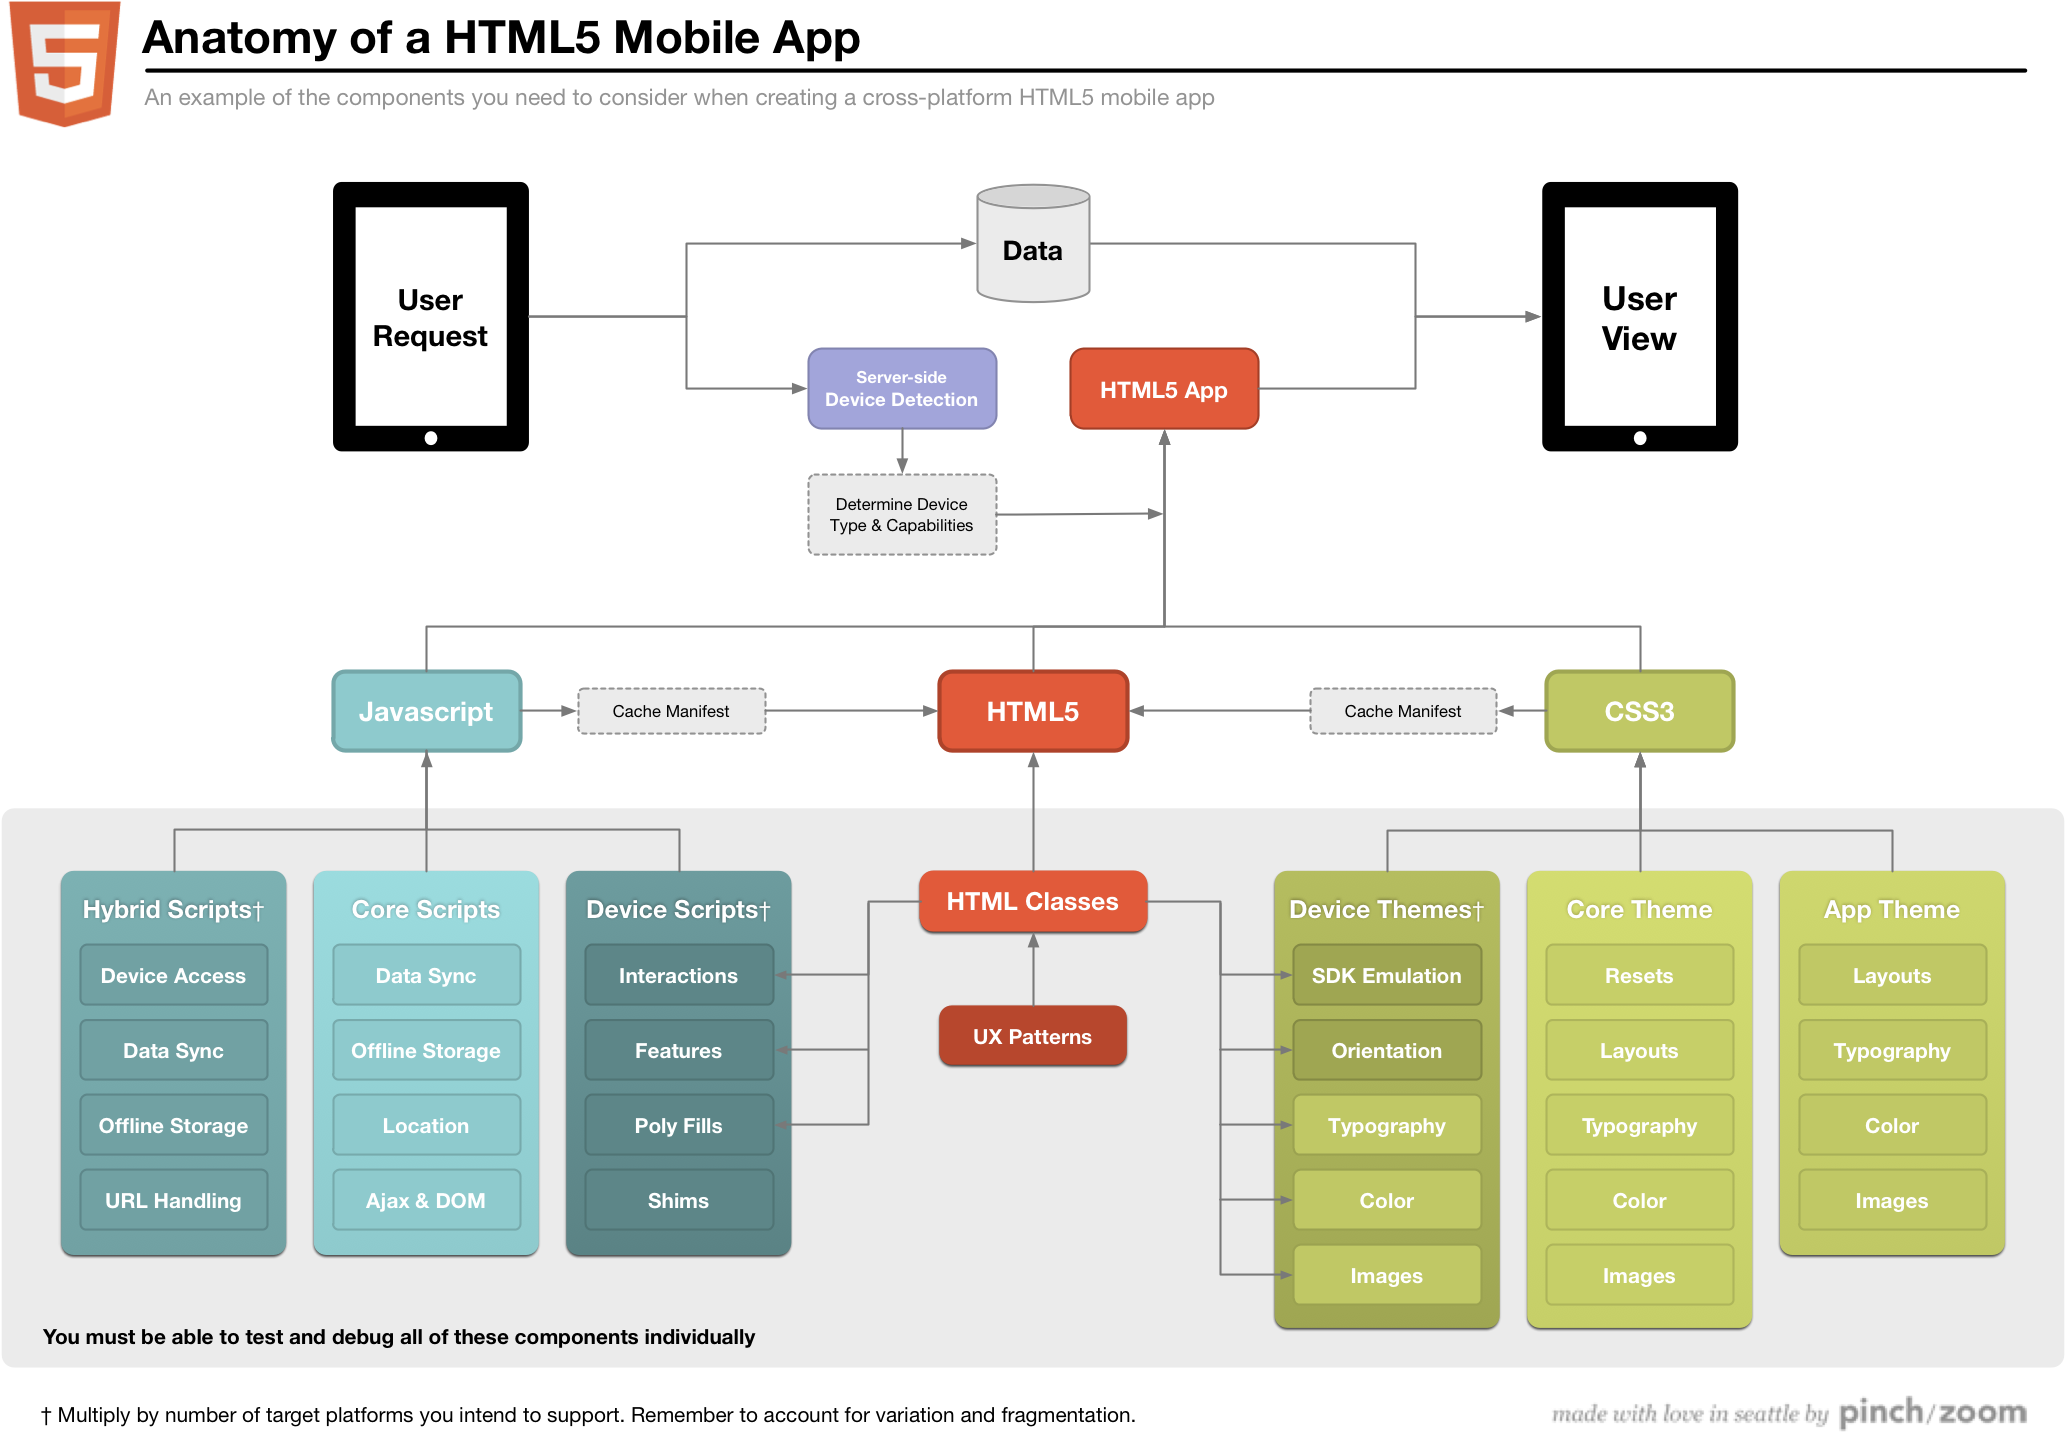
\includegraphics[width=\textwidth]{images/anatomy-of-a-html5-mobile-app.png}
  \caption{HTML5 Mobile Application Anatomy according to
    \cite{fling2011anatomy}.}
  \label{figure:anatomy-of-a-html5-mobile-app.png}
\end{figure}

In this chapter, I present tools, libraries, and techniques for
building modern web applications.

\section{Single-Page applications}
\label{section:single-page-applications}

In recent years, the movement from traditional interlinked documents
to interactive web applications has had a profound effect on the
architecture of web applications. Traditional web sites have
structured backend architectures often with a database layer, a layer
for business logic, and a layer for generating the HTML documents from
a template. The frontend usually uses \abbr{CSS} for layout and
styling and some JavaScript for enhancing forms or some interactive
components on a page.

These conventional three-tiered web applications often use an
\abbr{MVC} \cite{gamma1995design} framework for separating the data,
logic, and presentation layers in the backend. However, the latest
trend in web application development has been having only a simple
\abbr{REST} \cite{fielding2000architectural} API as a backend data
layer, and using a JavaScript MVC framework in the frontend. Thus the
whole application logic and presentation has moved to the client side,
with the backend only working as a data persistency layer.

Using modern JavaScript storage APIs (see
Section~\ref{section:datastorage}), even the data persistency and
application state layer can be in the client side, with backend only
working as an application and data delivery layer. In addition to the
client side data persistency, the storage APIs can be used to store
the user-specific application state.

Single-page applications might introduce bigger initial page load, but
after the startup, the network is only used when interacting with the
backend data API. This makes the applications faster and more
responsive, and minimizes the effects that unreliable networks have on
the application usage since separate page views do not require a new
document request.

\section{JavaScript MVC Libraries}
\label{section:js-mvc}

Due to the recent trend to move application logic from the backend to
the frontend, JavaScript code bases have grown into large applications
that need a proper modular structure. Several frameworks have been
developed to structure JavaScript applications into well-separated
modules and layers.

Many of the JavaScript application frameworks are derived from the MVC
architecture pattern adapting it to the design needs and requirements
of browser-based applications. Example frameworks include
Backbone.js\footnote{\url{http://backbonejs.org/}},
Spine\footnote{\url{http://spinejs.com/}},
batman.js\footnote{\url{http://batmanjs.org/}},
Knockout\footnote{\url{http://knockoutjs.com/}}, and
JavaScriptMVC\footnote{\url{http://javascriptmvc.com/}}.

One popular framework nowadays is Backbone.js, which I also chose for
the application described in
Chapter~\ref{chapter:methods}. Backbone.js is an open source
JavaScript framework providing the essential components and structures
for building large JavaScript applications. Backbone.js provides the
following components:

\begin{itemize}
\item \textbf{Model}

  Models provide the domain-specific data layer of the
  application. They provide data manipulation, persistency, and
  serialization methods as well as an event handling mechanism for
  data changes.

\item \textbf{Collection}

  Collections are ordered sets of models. They can be used to observe
  and manipulate models as a group. They can also be used to filter
  specific models for some purposes.

\item \textbf{Router}

  Routers provide methods for routing between pages of an application
  by observing and modifying the \abbr{URL}. URLs can be mapped to
  events and actions for client-side application navigation.

\item \textbf{History}

  The History utility is used together with Routers to handle the
  application navigation to preserve the back button functionality and
  the bookmarking of certain pages in the application.

\item \textbf{Sync}

  The Sync utility provides data synchronization to the backend.

\item \textbf{View}

  Views are structures that help organizing the user interface into
  logical parts. They usually observe certain models or collections
  for changes, and update themselves independently of each other when
  the underlying data changes. They are often used together with some
  templating library, such as
  Mustache\footnote{\url{http://mustache.github.com/}} or
  Handlebars\footnote{\url{http://handlebarsjs.com/}}.

\end{itemize}

\section{Responsive Design}

Responsive design is a way to design a web page to fit to varying
sizes of screens and devices. The traditional way to design a web page
is to compromise on a certain width based on the expected desktop
screen sizes of the target audience and to lay out the elements of the
page to the chosen width.

Using Media Queries (see Section~\ref{section:css}), we can provide
tailored layouts for different screen sizes. For example, we can swap
the images to smaller ones for mobile devices or hide some elements to
make the layout cleaner on small screens. This enables us to use the
same code base to target all devices and screens.

\section{Progressive Enhancement}
\label{subsection:progressive-enhancement}

Modern web sites and web applications are accessed with a huge variety
of devices and form-factors with varying capabilities, and supporting
all the possible browsers your users might have becomes a huge burden
on developers. New standards support and \abbr{APIs} in latest
browsers seem tempting and valuable, but having to support also
less-capable browsers prevent developers from using a single solution
for all browsers.

The goal of progressive enhancement is to provide universal access to
a web site or application no matter what capabilities the browser of
the user has. Parker et al. define the three key principles of
progressive enhancement \cite{parker2010designing}:

\begin{itemize}
\item Start with clear content and well-structured markup.
\item Maintain strict separation of layout and presentation.
\item Unobtrusively layer in advanced behavior and styling, with
  careful consideration of accessibility implications.
\end{itemize}

Often the design is started ``mobile first'' meaning that the simplest
and the most universal bottom layer of the application is designed for
the least-capable browsers with very little screen estate. This forces
the design to be simple and semantic, and filters out any extra markup
that is not needed for the semantic presentation of the content and
functionality. In addition, by designing first to browsers that might
not even have \abbr{CSS} support forces a clear separation of layout
and content as well as makes the clean markup easier to style and
enhance \cite{parker2010designing}.

Using feature detection (see Section~\ref{section:feature-detection}),
more layers are added on top of the clean markup. The objective is to
use unobtrusive JavaScript to enhance the markup to avoid breaking
parts of the page or the whole site with careless scripting. By using
feature detection, we ensure that we take the most out of the latest
browsers by using their full capabilities, and at the same time,
keeping the application accessible and functional in less-capable
browsers. This also makes the applications future-proof when browsers
are updated and new APIs and features are implemented in
them. \cite{parker2010designing}

\section{User Interface Libraries}

User Interface libraries help in developing mobile web applications
fast by providing finished and tested widgets and user interface
components that can be combined and configured easily. I present some
popular frameworks in the following sections.

\subsection{jQuery Mobile}

jQuery Mobile\footnote{\url{http://jquerymobile.com/}} is a client
side framework optimized for touch devices. The user interface is
based on HTML5 and the jQuery JavaScript
framework\footnote{\url{http://jquery.com/}}. The aim of the project
is to provide a progressively enhanced web framework for as many
devices as possible. Figure~\ref{figure:jquerymobile.png} shows
example components in the framework.

\begin{figure}[ht]
  \begin{center}
    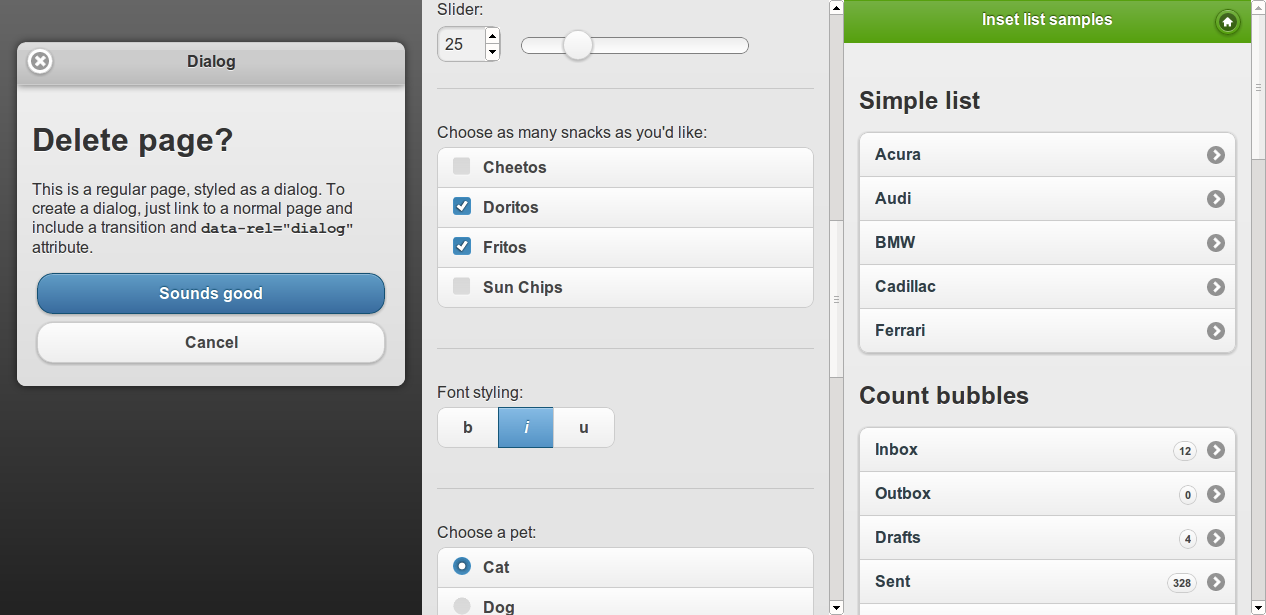
\includegraphics[width=\textwidth]{images/jquerymobile.png}
    \caption{jQuery Mobile user interface
      components. \url{http://jquerymobile.com/demos/1.0.1/}}
    \label{figure:jquerymobile.png}
  \end{center}
\end{figure}

jQuery Mobile is an open source project sponsored by large mobile and
media companies. The user interface is fully theamable and there are
several third-party extensions and widgets to the framework.

\subsection{jQTouch}

jQTouch\footnote{\url{http://jqtouch.com/}} is a lightweight open
source library for high-end smartphones and tablet devices. It only
supports the WebKit browser
engine \footnote{\url{http://www.webkit.org/}} used in iOS, Android,
Blackberry, and WebOS devices. It provides customizable themes and
user interface components, as well as helpers for handling touch
input. Figure~\ref{figure:jqtouch.png} shows example components of the
library.

\begin{figure}[ht]
  \begin{center}
    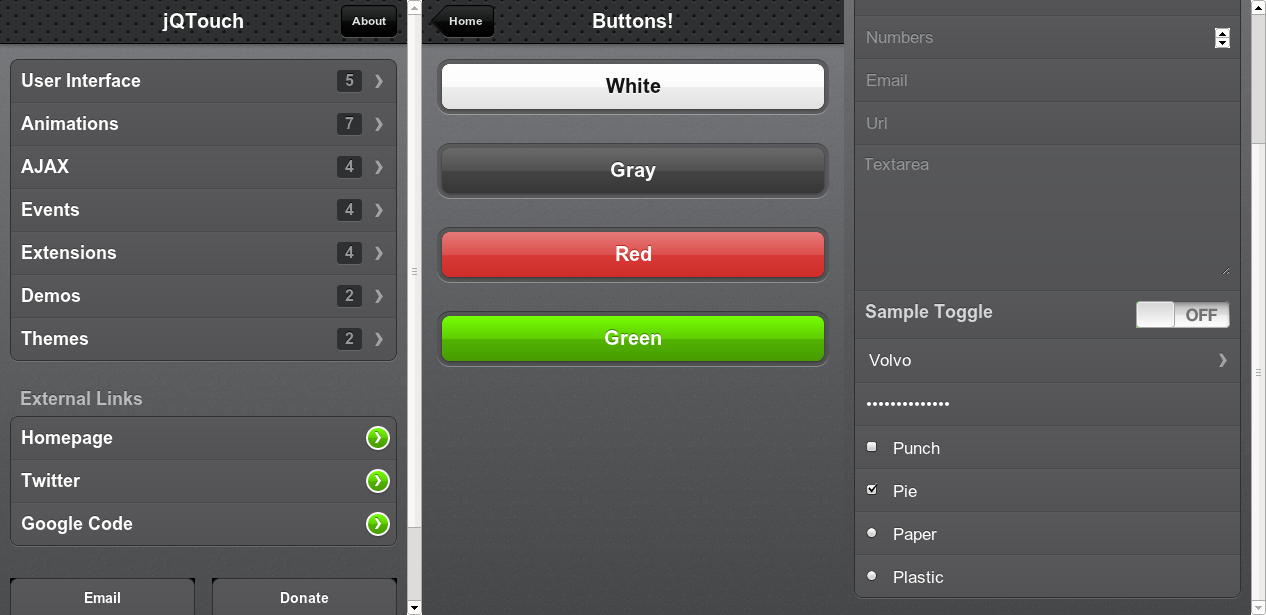
\includegraphics[width=\textwidth]{images/jqtouch.png}
    \caption{jQTouch user
      interface. \url{http://jqtouch.com/preview/demos/main/}}
    \label{figure:jqtouch.png}
  \end{center}
\end{figure}

\subsection{Sencha Touch}

Sencha Touch\footnote{\url{http://www.sencha.com/products/touch}} is
an open source HTML5 mobile web application framework for iPhone,
Android, and Blackberry devices. The framework is fully theamable and
comes with a large set of user interface components. It also provides
helpers for touch input handling. Figure~\ref{figure:sencha.png} shows
example components of the library.

\begin{figure}[ht]
  \begin{center}
    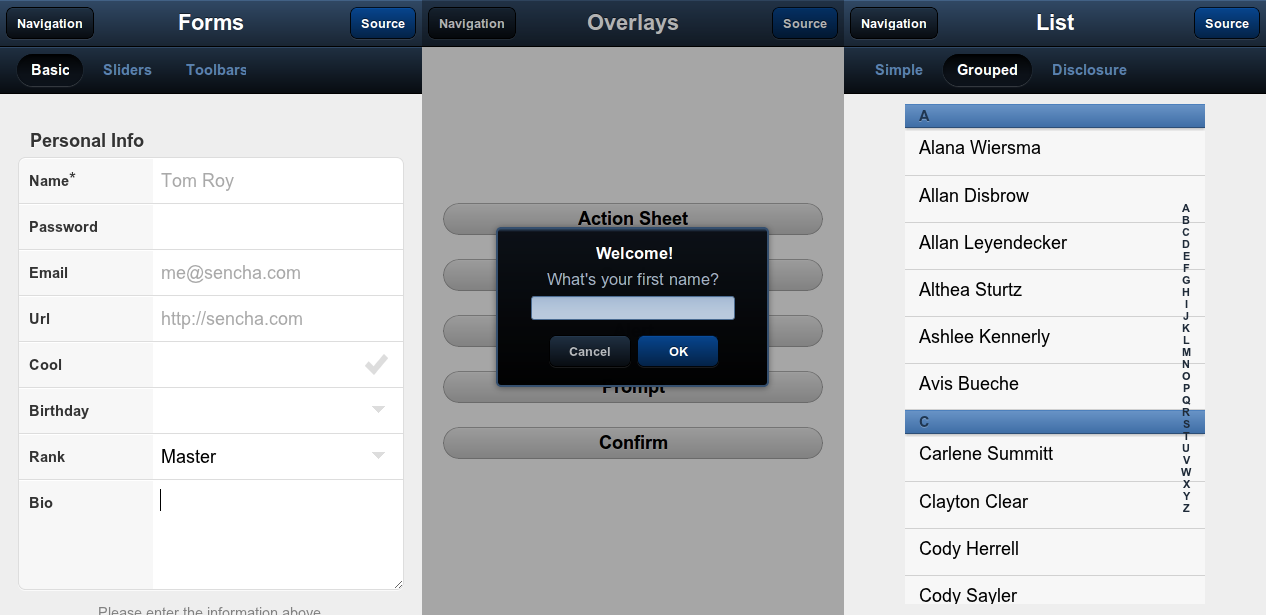
\includegraphics[width=\textwidth]{images/sencha.png}
    \caption{Sencha Touch user
      interface. \url{http://dev.sencha.com/deploy/touch/examples/kitchensink/}}
    \label{figure:sencha.png}
  \end{center}
\end{figure}

\section{Hybrid Applications}

Sometimes application stores can be a valuable marketing path, and
visibility in these stores can bring a lot of users to an
application. The stores also provide easy billing of applications
themselves, and solutions for in-app
billing. \cite{cortimiglia2011mobile}

Fortunately, modern smartphone and tablet platforms provide a user
interface component to embed a web browser view into a native
application. This web view component can be used to build parts or
even the whole application with web technologies. For example, the web
view can take the whole available screen space of the application, and
show a local HTML document together with local assets like CSS and
JavaScript files and images.

These applications that use a native web view wrapper with parts of
the application built with web technologies are called hybrid
applications. The level of native versus web technologies can vary,
and everything is possible from fully utilizing web technologies with
just a simple native wrapper to a native application with just a
simple static HTML document.

Several tools have been developed to build hybrid applications. One of
these is PhoneGap \footnote{\url{http://phonegap.com/}}, which is an
open source HTML5 application platform for building native
applications with web technologies. PhoneGap provides native wrappers
for all of the largest mobile platforms, and exposes extra JavaScript
APIs that are not accessible in normal web pages. These APIs are based
on the latest specifications, and they can be used to access device
functionality that has previously been inaccessible using JavaScript.

With tools like PhoneGap, developers can build native applications
using familiar web technologies with access to native features and
device APIs. These hybrid applications have only one code base that is
deployed for several smartphone platforms, and the applications can be
submitted to application stores.

\clearpage
\section{Performance Guidelines}
\label{section:performance-guidelines}

There are several web application performance best practices and
related guidelines. According to Souders \cite{souders2007high}, only
10--20\% of the end user response time is spent generating and
transferring the HTML document from the web server to the
client. Therefore, most of the optimization should be done in the
frontend for best improvement opportunities. Below I list the
performance guidelines defined by Souders \cite{souders2007high}.

\begin{itemize}

  % High Performance Web Sites

\item \textbf{Make Fewer HTTP Requests}

  According to Souders, 80--90\% of the end user response time is
  spent downloading components in a page other than the requested HTML
  page. Therefore, the simplest way to improve the response time is to
  reduce the number of HTTP requests needed to get all the required
  components.

  There are several ways to reduce the number of needed HTTP
  requests. Combining images into sprites, inlining images, or
  combining separate JavaScript and CSS files results in fewer
  components needed to download on a page.

\item \textbf{Use a Content Delivery Network}

  As web applications are deployed and become accessible worldwide,
  latency might become an issue for users far from the application's
  web servers. Geographically distributed servers allow for serving
  the application as close to the user as possible.

\item \textbf{Add an Expires Header}

  Avoiding a HTTP request altogether is the best option for reducing
  the response time when downloading the components in a page. Good
  caching strategies help browsers to know which resources are valid
  and for how long until they should be updated.

  The Expires header in HTTP tells the client how long a resource is
  valid, and especially far future Expires headers reduce the need for
  downloading and updating the components in a page after the initial
  download.

\item \textbf{Gzip Components}

  Compressing HTTP responses is an easy and effective way to reduce
  the size of the data needed to transfer across the
  network. Compression is supported widely in web browsers and the
  impact of reduced response sizes is huge. Using Gzip, the response
  size is reduced generally about 70\%.

\item \textbf{Put Stylesheets at the Top}

  Putting the CSS files to the top of the document allows the page to
  load progressively and the browser to show visual feedback to the
  user as early as possible.

\item \textbf{Put Scripts at the Bottom}

  Because scripts block parallel downloads, they should be included to
  the page after all other resources. They also block progressive
  rendering of all content below them in the HTML document, and should
  therefore be at the bottom of the document.

\item \textbf{Avoid CSS Expressions}

  CSS expressions are a way to dynamically set CSS properties in
  Internet Explorer by evaluating a JavaScript code in a
  stylesheet. However, despite the obvious upsides, the expressions
  are evaluated at such a high frequency that they negatively impact
  the performance.

\item \textbf{Make JavaScript and CSS External}

  There are performance tradeoffs between making JavaScript and CSS
  external versus inlining them in the HTML document. In the typical
  case, however, making them external enables the browser to leverage
  the HTTP caching semantics and thus reduces the needed network
  transfer.

\item \textbf{Reduce DNS Lookups}

  Apart from cached \abbr{DNS} lookups, the browser typically needs
  20--120 milliseconds to look up the \abbr{IP} address for a given
  hostname. The cache lifetime of a lookup depends on the \abbr{TTL}
  value of the DNS record and having the components of a page
  distributed across several domains might accumulate into a
  noticeable response time.

  There is also a trade-off between unique hostnames and allowed
  parallel connections and therefore these settings should be
  configured based on the application architecture and needs.

\item \textbf{Minify JavaScript}

  Because JavaScript is an interpreted language that must be sent to
  the web browser as source code, minifying the code reduces the
  required network transfer. Minifiers and obfuscators optimize the
  size of the source code by stripping extra whitespace and comments
  as well as renaming variables and function names to shorter ones
  without changing the interpreted behavior of the code.

\item \textbf{Avoid Redirects}

  Rerouting any component in a page takes time, and avoiding any kind
  of redirects improves the response times.

\item \textbf{Remove Duplicate Scripts}

  Including a resource several times serves no purpose but is actually
  quite common. Developers should make sure to include resources only
  once.

\item \textbf{Configure ETags}

  \abbr{ETags} are a mechanism in HTTP for servers and browsers to
  validate cached resources. The typical default values set by
  commonly used web servers might hurt performance, and should thus be
  configured properly to address the application architecture and
  needs.

\item \textbf{Make Ajax Cacheable}

  Highly dynamic web sites have a lot of \abbr{Ajax}
  \cite{garrett2005ajax} functionality, and developers should make
  sure all the requested URLs for data fetching follow the performance
  best practices such as having proper caching in place.

\end{itemize}

In addition to the performance rules \cite{souders2007high}, Souders
also specifies additional techniques to improve performance
\cite{souders2009even}:

\begin{itemize}

  % Even Faster Web Sites

\item \textbf{Splitting the Initial Payload}

  Nowadays, web sites include a lot of resources and JavaScript
  functionality, but only a small part of the downloaded components
  are used in the typical use cases of the application. Splitting the
  resources into bundles that can be lazily downloaded when first
  needed reduces the initial payload needed to transfer on application
  startup.

\item \textbf{Loading Scripts Without Blocking}

  Most browsers block the downloads of other resources when scripts
  are being downloaded and executed. There are several ways to
  circumvent this behavior to allow browsers download scripts in
  parallel with other resources as well as with other script files.

\item \textbf{Coupling Asynchronous Scripts}

  Related to the previous item, when using parallel downloads with
  scripts that are dependent on each other, race conditions might
  occur due to the varying order of download and execution. Therefore,
  asynchronous scripts dependent on each other should be coupled to
  preserve the correct order of execution.

\item \textbf{Positioning Inline Scripts}

  Inline scripts do not introduce an HTTP request, but they can still
  block parallel downloads of other resources and they might affect
  also the progressive rendering of the page. With the correct
  positioning of the scripts, these problems can be handled properly.

\item \textbf{Writing Efficient JavaScript}

  After networking, the obvious place to optimize the runtime speed of
  a web application is the JavaScript code.

  Because the whole user interface and the JavaScript code run in the
  same browser thread, there can be only one thing happening at a
  time. Long running functions block the user interface from updating
  and can result in bad user experience.

  Splitting the running code into properly sized chunks, appropriately
  leveraging the asynchronous patterns of JavaScript in the
  application architecture, understanding the details and slow parts
  of the DOM API, and using several JavaScript programming best
  practices can result in big improvements in the perceived
  application performance. \cite{zakas2010high}

\item \textbf{Scaling with Comet}

  For real-time data-driven applications, there are various
  optimization techniques related to optimizing the constant data
  transfer between the server and the client. The collection of there
  various technologies is unofficially called Comet.

\item \textbf{Going Beyond Gzipping}

  Although Gzipping is widely supported in web browsers, there are
  cases when it is not supported or when the support is not
  indicated. Stripping extra content such as unneeded whitespace and
  comments reduces the payload size for uncompressed responses. There
  are also ways to detect Gzip support if the client does not directly
  indicate that.

\item \textbf{Optimizing Images}

  Images typically tend to account for a large portion of the page
  weight, and since the page weight is highly correlated to the
  response time, images are a natural target for optimization. There
  are several ways to optimize images either with lossy or lossless
  conversions.

\item \textbf{Sharding Dominant Domains}

  By tuning the amount of unique hostnames used for serving all the
  resources of an application, parallel downloads can be better
  leveraged. Also, by using HTTP 1.0 with proper Keep-Alive headers or
  HTTP 1.1 with proper persistent connections the parallel downloads
  can be tuned for better performance.

\item \textbf{Flushing the Document Early}

  Some web application frameworks allow flushing parts of the document
  to the user before the whole document is generated. This enables
  progressive rendering and gives faster feedback to the user and thus
  improves the perceived performance.

\item \textbf{Using Iframes Sparingly}

  Iframes enable developers to embed a separate HTML document inside
  another document. They are useful in sandboxing external documents
  in the same view, but the \texttt{iframe} element is the most
  expensive DOM element related to the page performance.

\item \textbf{Simplifying CSS Selectors}

  There are several ways to choose elements in CSS stylesheets to
  apply the defined properties to. Some selectors are faster than
  others and some have terrible performance.

\end{itemize}

%\chapter{Research Question}
\label{chapter:research-question}

\chapter{Methods}
\label{chapter:methods}

\section{Qt Developer Days 2011 Conference Schedule Application}
\label{section:devdays}

The Qt Developer
Days\footnote{\url{http://qt.nokia.com/qtdevdays2011/}} is a
conference for developers using the Qt cross-platform application and
user interface framework\footnote{\url{http://qt.nokia.com/}}. We
created a mobile web application with contextual and personalized
session information and daily schedule for the conference.

\subsection{Requirements}

\begin{itemize}
\item usage context: conference (network problems expected)
\item target audience: mobile developers (knowledgeable audience)
\item target devices: iPhone, Android phones, WP7, iPad (also tested
  on more devices)
\item personalized application: session favorites
\item contextual UI: showing coming/ongoing favorite sessions, showing
  current time in agenda, opening agenda in the current day
\item floor maps with rooms
\item session feedback form
\end{itemize}

\subsection{Application Architecture}

\begin{figure}[ht]
  \begin{center}
    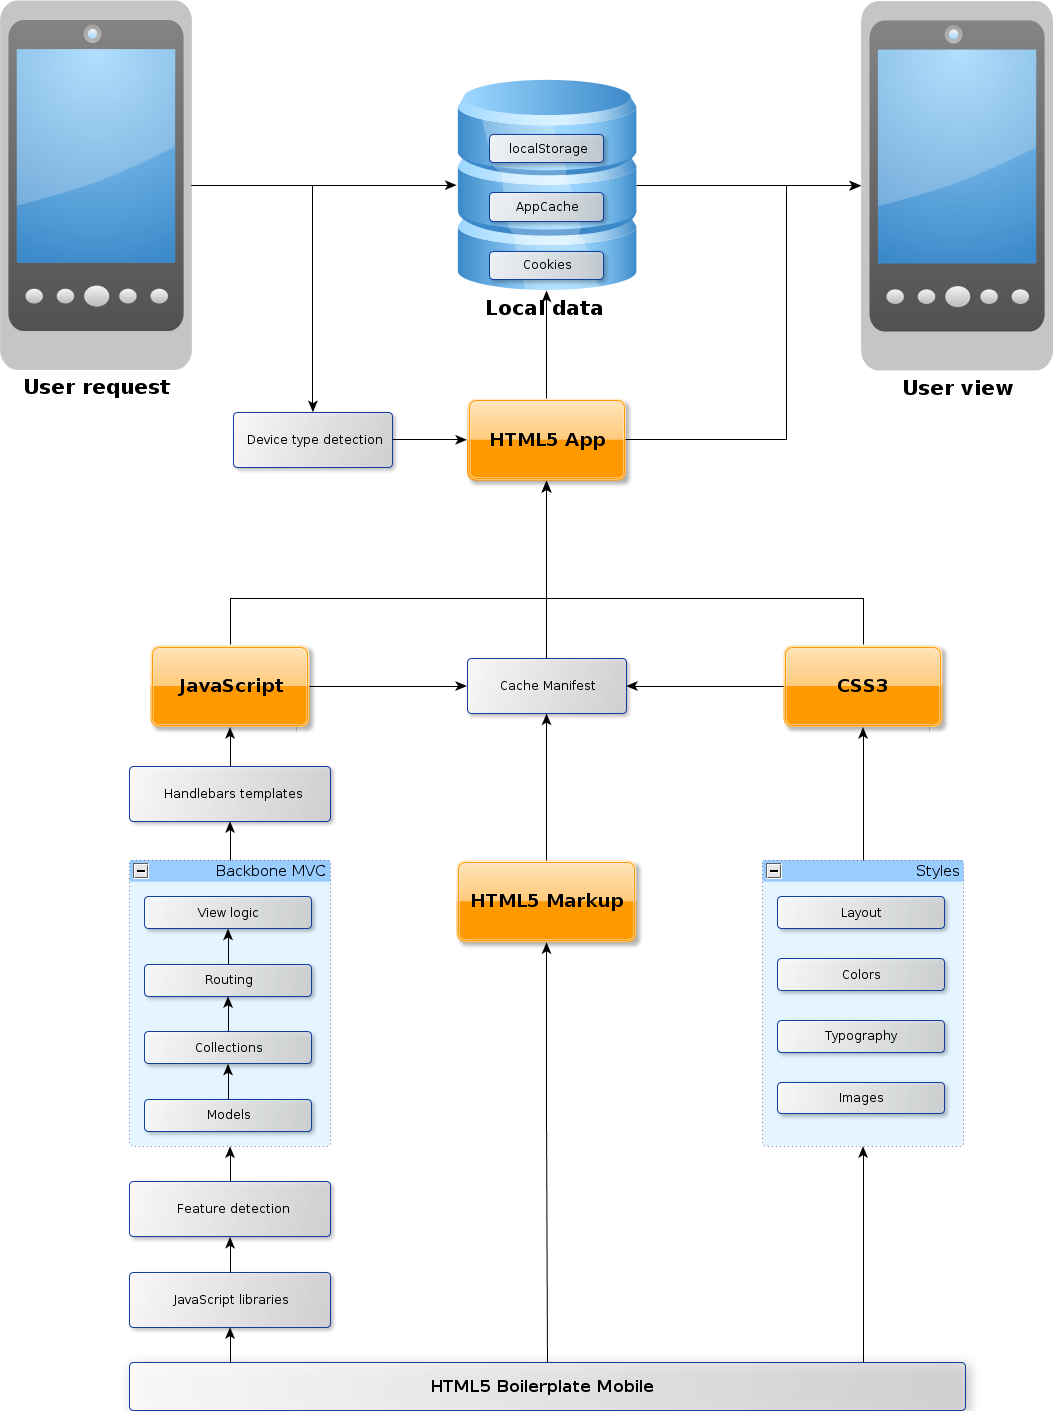
\includegraphics[width=\textwidth]{images/devdays.png}
    \caption{Conference schedule application architecture.}
    \label{figure:devdays.png}
  \end{center}
\end{figure}

The conference
schedule\footnote{\url{http://m.qtdevdays2011.qt.nokia.com/}} is a
single-page application (see
Section~\ref{section:single-page-applications}) with a lightweight
backend written in Python using the Django Web
Framework\footnote{\url{https://www.djangoproject.com/}}.

The backend provides the static assets (JavaScript, \abbr{CSS},
images, etc.) and an \abbr{API} for persisting session feedback to a
MySQL\footnote{\url{http://www.mysql.com/}} relational database. It
also generates the HTML5 AppCache (see Section~\ref{section:appcache})
offline cache manifest file based on the categorized device type.

The frontend is a JavaScript application written using the
Backbone\footnote{\url{http://backbonejs.org/}} \abbr{MVC} framework
(see Section~\ref{section:js-mvc}). Other used JavaScript libraries
include Underscore\footnote{\url{http://underscorejs.org/}} for data
manipulation, jQuery\footnote{\url{http://jquery.com/}} for \abbr{DOM}
API abstraction, Handlebars\footnote{\url{http://handlebarsjs.com/}}
for templating, and
Modernizr\footnote{\url{http://www.modernizr.com/}} for feature
detection. The HTML5 Mobile
Boilerplate\footnote{\url{http://html5boilerplate.com/mobile}} was
used as an initial markup structure for the application. The
architecture of is shown in Figure~\ref{figure:devdays.png}. Wireless
networks can be unreliable in conference settings, so offline support
was also added using several different JavaScript techniques and HTML5
APIs.

The application was designed for touch screens on various platforms
and screen sizes. The layout adjusts to the available space and
provides rich interactive components. Integration to social networking
services was also added as an additional functionality.

\fixme{add screenshots on different devices (at least phone and tablet}

\section{JSONCache JavaScript Library}
\label{section:jsoncache}

JSONCache is a lightweight JavaScript library for fetching \abbr{JSON}
data in unreliable networks. The library was designed especially to
handle unreliable mobile networks with connection problems and short
interruptions. The goal is to avoid networking as long as possible and
failing gracefully if the network connection is not stable.

JSONCache provides two main functionalities: data caching and
attempting to fetch the data multiple times.

The caching layer uses the client side localStorage (see
Section~\ref{section:datastorage}) cache of \abbr{HTML5}. Data
requests can be done using the JSONCache \abbr{API} which always
checks the local cache first before opening any network
connections. If the data is already in the cache, the cached data is
checked for validity and if the data has not been expired, it is
returned immediately. If the data is not in the cache or it has been
expired, a new network request is made and the received data is cached
and returned. The expiration time of a data item can be configured in
the library settings.

JSONCache also tries to fetch the data multiple times to handle small
interruptions in network connections. \fixme{add example and explain
  that it is very common}. If a data fetch fails, a new fetch is
issued after a timeout (defined in the configuration). On subsequent
attempts the timeout is increased, and after a defined number of
attempts the fetch error is issued.

Figure~\ref{figure:jsoncache-demo.png} shows an interactive demo of
the JSONCache library. The
demo\footnote{\url{http://kpuputti.github.com/JSONCache/demo/index.html}}
simulates the caching and fetching functionality of the library by
simulating an unreliable network based on the configuration.

\begin{figure}[ht]
  \begin{center}
    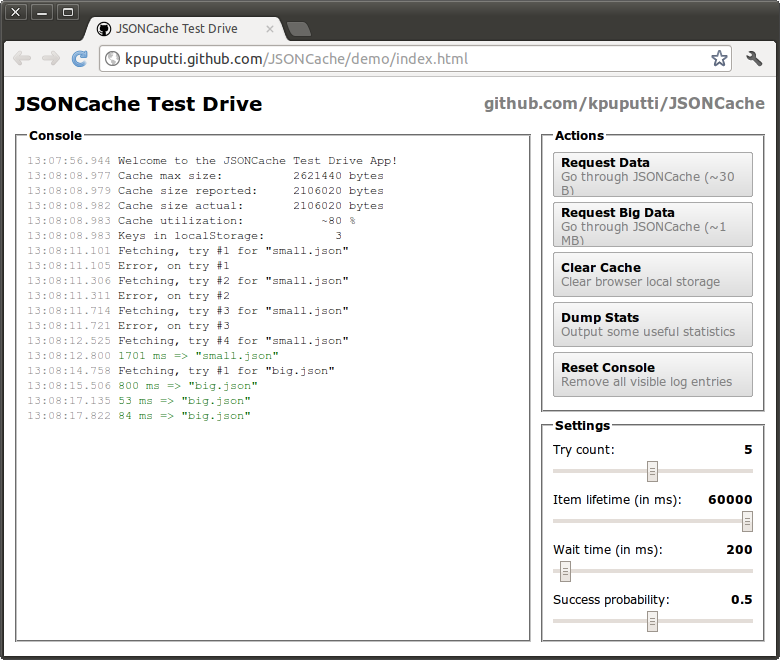
\includegraphics[width=\textwidth]{images/jsoncache-demo.png}
    \caption{Interactive JSONCache demo.}
    \label{figure:jsoncache-demo.png}
  \end{center}
\end{figure}

\chapter{Results: What Was Good and Where Were the Compromises}
\label{chapter:results}

\section{Targeting Different Platforms}
\label{section:targeting-platforms}

Despite the web browser being the unified environment for different
platforms, there are lots of differences between various devices. The
form factors vary from tiny mobile screens to touch screen tablets and
desktop monitors and each device and platform has its own feature
set. There are also known bugs in the browsers that have to be
handled.

Therefore, means to detect the user's device are needed. Here we
present two such means: device detection and feature detection. Both
of these were used in our conference application.

\subsection{Device Detection}
\label{subsection:device-detection}

The User-Agent (\abbr{UA}) \abbr{HTTP} header contains detailed
information of the web browser and platform where the request
originates. As we can see from Table~\ref{table:user-agents}
(\fixme{Check table ref number}), we can extract platform and browser
specific information from the UA header.

\begin{table}
  \begin{tabular}{ l | l | p{7cm} }
    \textbf{Device} & \textbf{Platform} & \textbf{User-Agent} \\ \hline
    Samsung Nexus S & Android 2.3.4 & Mozilla/5.0 (Linux; U; Android 2.3.4; en-us; Nexus S Build/GRJ22) AppleWebKit/533.1 (KHTML, like Gecko) Version/4.0 Mobile Safari/533.1 \\ \hline
    Apple iPhone & iOS 3.1.3 & Mozilla/5.0 (iPhone; U; CPU iPhone OS 3\_1\_3 like Mac OS X; de-de) AppleWebKit/528.18 (KHTML, like Gecko) Version/4.0 Mobile/7E18 Safari/528.16 \\ \hline
    Apple iPad & iOS 5.0 & Mozilla/5.0 (iPad; CPU OS 5\_0 like Mac OS X) AppleWebKit/534.46 (KHTML, like Gecko) Mobile/9A334 \\ \hline
    Unknown & Android & Opera/9.80 (Android; Opera Mini/6.5.26571/26.1023; U; de) Presto/2.8.119 Version/10.54 \\ \hline
  \end{tabular}
  \label{table:user-agents}
  \caption{Example User-Agent strings.}
\end{table}

In the conference application, device detection was used in the
backend to provide a different offline AppCache manifest to different
device groups. The detection was also used in defining the assets to
be preloaded in the application. The devices were divided into four
categories based on the rules defined in
Table~\ref{table:device-detection-rules} (\fixme{Check table ref
  number}). There were serious limitations in this approach, and
compromises had to be made.

First, there is no way to surely know if the device actually is what
it reports itself to be. Second, the most important thing to know when
generating the screen specific assets in the manifest file would have
been the screen size. However, this information is not present in the
UA header. We could have listed all the assets for all the devices,
but then the list of offline assets would have grown too much and, for
example, have large images also for older mobile phones.

Despite the drawbacks, the received advantages of this approach
outweighed the possible compromises. The worst that could happen was
that the device was wrongly classified and the proper resources were
not downloaded for offline use.

\begin{table}
  \begin{tabular}{ l | l }
    \textbf{Rule} & \textbf{Device Type} \\ \hline
    'iPad' in UA & highres \\
    'iPhone' in UA & iphone \\
    'Android 3' in UA & highres \\
    'mobile' (case insensitive) in UA & mobile \\
    'MIDP' in UA & mobile \\
    'Opera Mobi' in UA & mobile \\
    'Opera Mini' in UA & mobile \\
    otherwise (desktop computer) & highres
  \end{tabular}
  \label{table:device-detection-rules}
  \caption{Device type detection rules.}
\end{table}

Getting platform and browser information from the UA header might look
tempting and useful, but it is considered a bad practice to detect a
device from it and provide device specific bug fixes or additional
features. The header can easily be changed and some browsers or
browser plugins even provide preconfigured values for certain browsers
or devices for spoofing. Also, the device specific bug fixes might
become obsolete with platform updates, and the application might break
due to invalid expectations. This is why feature detection is
generally the recommended option whenever possible.

\subsection{Feature Detection}

Feature detection is an important concept in Progressive Enhancement
design (See Section~\ref{subsection:progressive-enhancement}). A lot
of the HTML5 related JavaScript APIs are still unsupported in several
platforms, but browser developers are constantly filling the
gaps. Therefore, it is important to check whether a certain feature is
supported and provide graceful fallback mechanisms for browsers
lacking the functionality.

Doing runtime feature detection provides the possibility to give
additional functionality to modern browsers and instant support for
devices that add the feature support in the lifetime of the
application. In the conference application (\fixme{ref needed?}), we
used the Modernizr feature detection library (\fixme{already ref
  earlier, add bib entry?}) to check for HTML5 features.

For example, the user could add sessions to his or her favorites by
clicking the star in the agenda or on the session details view
(\fixme{add screenshot?}). The favorites were then listed on the home
view together with information about the time left for them to begin.

We used HTML5 localStorage for storing the favorites in the user's web
browser. By using Modernizr, we detected localStorage support and
showed the favorite stars only in browsers that supported the
functionality. For all other browsers, the stars were simply hidden
and users could not add favorites. We could have also provided a
fallback mechanism for persisting the favorites to the backend, but
for simplicity and because we targeted mostly modern platforms, this
approach was considered as reasonable.

\section{Targeting Different Screens}
\label{section:targeting-screens}

Probably the biggest difference in various devices and form factors is
the screen size, resolution, and dimensions. Web applications should
adjust to the available space and flexible handle screen orientation
and window size changes.

First, to target mobile and tablet platforms, the viewport meta
information should be indicated in the document. The following tag was
used in the conference application:

\begin{verbatim}
<meta name="viewport" content="width=device-width,
                               initial-scale=1.0">
\end{verbatim}

The viewport meta tag was first introduced in Apple's iPhone and
afterwards ported to other platforms, such as Android. The possible
configuration options and default values might vary between
platforms. Values accepted by Android are shown in
Table~\ref{table:viewport-meta} (\fixme{Check table ref number})
\citationneeded. iOS devices also support these same properties.

\begin{table}
  \begin{tabular}{ l | l | p{5cm} }
    \textbf{Property} & \textbf{Description} & \textbf{Value} \\ \hline
    height & Height of the viewport. & pixel value or 'device-height' \\
    width & Width of the viewport. & pixel value or 'device-width' \\
    initial-scale & Initial zoom level. & float value (0.01--10) \\
    minimum-scale & Minimum zoom level. & float value (0.01--10) \\
    maximum-scale & Maximum zoom level. & float value (0.01--10) \\
    user-scalable & Enables/disables zoom. & 'yes' or 'no' \\
    target-densitydpi & Visual pixel density. & dpi value, 'device-dpi', 'high-dpi', 'medium-dpi', or 'low-dpi' \\
  \end{tabular}
  \label{table:viewport-meta}
  \caption{Viewport meta tag configuration for Android.}
\end{table}

If we do not set the viewport configuration tag, the device uses its
own default values for the properties. For example, the default value
for the width property is 980 pixels in iOS \citationneeded, which is
clearly defined for web sites targeting desktop browsers. Without
setting this value to something smaller and more appropriate in a
mobile context, the whole application is very wide and has small and
unreadable text in the initial zoom level.

In the viewport configuration we used for the conference application
(as defined above), we set the viewport width to 'device\_width'. This
makes the application width to adjust to the visual pixels of the
device screen and works well with screens of different sizes and
dimensions. The only other viewport property we set is the initial
scaling. This is set to 1.0 to force the browser to render the
application without any initial zooming.

In addition to the viewport configuration, we used media queries
\citationneeded to use better background images for high resolution
screens. We also dynamically set the map view (\fixme{Add
  screenshot?}) images based on the screen dimensions so that we could
provide smaller images for smaller screens and high resolution images
for tablets and other devices with larger screen estate.

\section{Handling Different Orientations}

As shown in the previous section, screen sizes and dimensions vary
between devices. In addition to handling different resolutions and
dimensions, we must also handle screen orientation changes. The width
and height of the touch screens are usually different, and the user
can hold the device either in portrait or in landscape mode and in any
point switch between these two.

In the conference application, we wanted to have different header and
footer background images for different orientations. We also needed to
redraw the agenda view when the screen width changes since the items
on the schedule needed to be dynamically positioned to the available
space.

Mobile browsers trigger an 'orientationchange' event whenever the
device orientation changes. We listened to this event, inferred the
orientation from the screen dimensions, and executed the wanted
functionality for the event. We also had to do a fallback for Mobile
\abbr{IE} browser to listen to the window resize event because the
browser does not support the orientation change event.

\section{Handling Mobile Networks}
\label{section:handling-networks}

One of the biggest problems in mobile web applications is the often
slow and unreliable network. Our conference application was designed
for a context where the application cannot trust on the networking but
should still manage to handle interactions and persist application
state. Also being a conference where people come from around the
world, the network data transfer cost might be surprisingly high, and
thus bandwidth should be saved whenever possible.

\subsection{Minimizing Data Transfer}

The best approach to minimize data that needs to be transferred is to
avoid the transfer whenever possible, for example, with proper
caching. However, with initial download or with dynamic data, the
second best option is to minimize the size of the data needed to be
transferred.

First, we made sure the data was minimized and compressed with
Gzip. Second, using \abbr{JSON} instead of \abbr{XML} in \abbr{Ajax}
requests saves bandwidth and needed effort of the browser to process
the data. Third, using the offline manifest ensured that the
application assets and data needed to be downloaded only once, and
using localStorage we could store the application state locally to the
browser avoiding the network completely.

\subsection{Caching}

Caching on different levels of the application stack is one of the
most important optimizations that should be done. Caching can be done
in the client side using HTML5 APIs, on the HTTP level letting the
browser handle it complying to the HTTP caching header semantics, or
in various levels of the backend application stack.

In the conference application, we put the most focus on the HTTP
caching. Following the performance guidelines specified in
Section~\ref{section:performance-guidelines}, we created unique
\abbr{URLs} for all different versions of all static resources
(images, CSS, JavaScript, and AppCache manifest files) and set a far
future expires header for them. This way we could tell the browser to
cache all resources as far as possible and updating the resources was
handled by changing the version number in their corresponding URLs.

In addition to the HTTP-level caching, using the AppCache manifest
file told the browser to cache all needed resources to a more
persistent offline cache, which minimized needed downloads on
application startup if the resources were already in the cache.

Client side caching was used in saving the user specific state in the
conference application and experimented with the JSONCache library
specified in Section~\ref{section:jsoncache}. Using localStorage, we
can persist data in the browser and avoid networking if the cached
data is still relevant.

JSONCache handles the localStorage caching automatically, with only
user configuration needed for setting the data lifetime. Every time
the data is rerequested, the local cache is checked first, and
networking can be avoided altogether.

\subsection{Preloading}

One way to prevent \abbr{UI} slowness due to flaky networks is to
preload resources and data that is expected to be used later on. In
the conference application we predownloaded background images and
other graphics in the application initialization.

For example, downloading the header and footer background images for
both orientations made the device orientation change more responsive
because otherwise the browser would have started to download the
images after the orientation had already changed. With preloaded
images the browser just had to switch the image and render it
instantly without any networking.

\subsection{Offline Support}

Using HTML5 AppCache offline manifest file and storing application
state to localStorage, we provided full offline compatibility for the
conference application. With the offline manifest, we specified the
needed resources for all device types as categorized by the rules
defined in Section~\ref{subsection:device-detection}. The offline
cache also made subsequent application startups faster since the cache
is more persistent than the HTTP cache in browsers.

The offline support was especially critical for the conference
application since the conference had indeed very bad wireless network.
Without the offline support, users would not have been able to check
the session schedule during the conference.

However, the only thing needing the network was the session feedback
functionality. The application had a feedback form for all sessions,
and the submitted data was persisted in the backend. In offline mode,
this functionality was not available. Going further, we could extend
the offline support by saving the given feedback, for example, to
localStorage and sending it later to the backend server when the
network connection is open again.

\subsection{Handling Interruptions}

Small interruptions are common in mobile networks \citationneeded. For
example, the user might have a stable network connection, but after
walking into an elevator the connection drops for a moment. Then after
exiting the elevator the device reconnects to the
network. Applications should expect these interruptions and should not
fail immediately with brief interruptions in flaky networks.

JSONCache library introduced in Section~\ref{section:jsoncache} had a
functionality to overcome these issues. The library tries to download
the requested data multiple times, and fails only when the configured
maximum attempt count is reached. With every iteration, a timeout is
set for a new request, and the timeout is increased after each failed
attempt. This approach works very well, and together with localStorage
caching lets data updates circumvent small network interruptions
failing only when the network connection seems to be completely down.

\section{Animations}
\label{section:animations}

Animation and transitions, if not overused, can be a valuable addition
to the \abbr{UX} of an application. For example, having a simple
sliding animation between different views makes the application more
uniform and pleasing to the eye.

There are several ways to animate elements in a web application. The
simplest is to use \abbr{CSS3} animations. However, the performance of
the animations is not yet good enough for a cross-platform mobile
application. We tried to animate the view changes in our conference
application, but even a simple cross-fade did not have good enough
performance in all target platforms.

Using progressive enhancement techniques (see
Section~\ref{subsection:progressive-enhancement}) we could have
provided enhanced experience for the platforms that support animations
well, but only iOS devices performed well enough, so for simplicity we
did not use any animations.

\section{Following JavaScript Best Practices}
\label{section:js-best-practices}

\subsection{JSLint}

JSLint\footnote{\url{http://jslint.com/}} is a code quality tool for
JavaScript. There are several JavaScript features that are suboptimal
for performance or code maintainability. JSLint also checks for
JavaScript syntax and convention violations, which is valuable because
the code will be sent in the source form to be interpreted by the
browser.

We had automatic JSLint checking integrated in the Emacs
\citationneeded editor that we used for all JavaScript programming,
which helped to notice common errors as early as possible and made the
code cleaner.

\subsection{Lazy initialization}

Postponing work as long as possible is a valuable optimization
technique. In lazy initialization we minimize initialization work in
application startup to render the initial view fast. We then
initialize additional views only when they are requested.

Implementing lazy initialization needs more work than simply doing all
initialization work in the application startup, but the received
benefits are worth the extra effort. In the conference application we
tried to postpone all work to be done as late as possible and doing as
little work as possible for faster execution.

\subsection{Efficient DOM Manipulation}

\begin{itemize}
\item DOM manipulation is slow
\item Using document fragments
\item Minimizing reflows
\item \cite{zakas2010high}
\end{itemize}

\subsection{Efficient Event Handling}

\begin{itemize}
\item Event delegation
\item \cite{zakas2010high}
\end{itemize}

\section{Performance Analysis}
\label{section:performance-analysis}

We made a quantitative analysis of the conference application
performance by using two different tools: YSlow and Page Speed. These
tools analyze the web performance practices of a web page and provide
optimization guidelines. Many of the rules used in these tools are
derived from or based on the guidelines defined by Souders
\cite{souders2007high, souders2009even} and specified in
Section~\ref{section:performance-guidelines}.

\subsection{YSlow}

YSlow is a website analyzer originally developed by Steve Souders. It
checks the website against the rules defined in
Section~\ref{section:performance-guidelines}.

\fixme{Add YSlow results screenshot}

\subsection{Page Speed}

Page Speed \citationneeded is an open-source project by Google for
analyzing and optimizing web site performance best practices. We used
the Google Chrome browser extension to analyze the conference
application against the performance rules defined in Page Speed. The
results are pictured in Figure~\ref{figure:devdays-pagespeed.png}.

\begin{figure}[ht]
  \begin{center}
    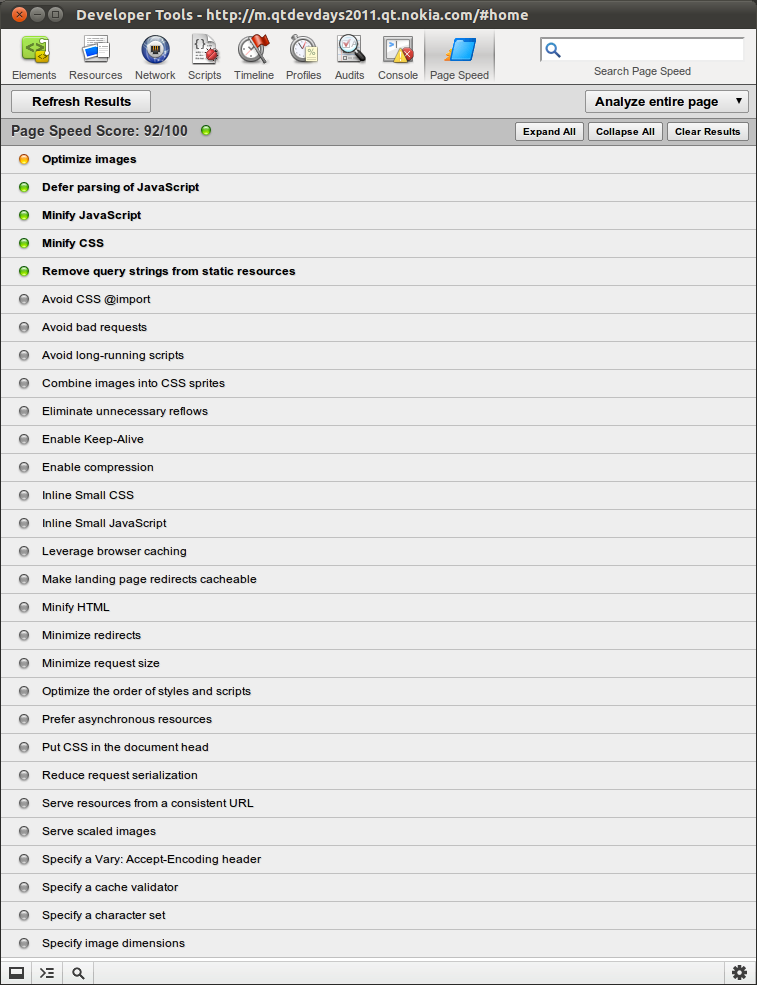
\includegraphics[width=\textwidth]{images/devdays-pagespeed.png}
    \caption{Page Speed results for the conference application.}
    \label{figure:devdays-pagespeed.png}
  \end{center}
\end{figure}

We were very happy with the Page Speed score of 92 out of 100. A lot
of the performance rules analyzed by Page Speed are similar to the
guidelines listed in Section~\ref{section:performance-guidelines}, but
there are also additional rules.

The only real problem in the score was the 'Optimize Images' rule. We
had not optimized the images used in the application, but instead used
the images provided by the designers. Going further, we could have
saved a lot or bandwidth by optimizing the images with tools such as
Pngcrush\footnote{\url{http://pmt.sourceforge.net/pngcrush/}}.

Of the other notes in the results, 'Defer parsing of JavaScript' could
have been avoided by adding a 'defer' attribute to all the script tags
in the document. The reason for this rule is that scripts block page
rendering as defined in
Section~\ref{section:performance-guidelines}. However, since we
followed the guideline 'Put Scripts at the Bottom', this rendering
issue is avoided. The only script in the document head was Modernizr,
which must be included before the page is parsed because it creates
the essential HTML5 tag support for older browsers and must do so
before the tags are parsed.

The 'Minify JavaScript' note was probably due to the Handlebars
templating library not being minified. All the JavaScript libraries
were included in their minified form, but Handlebars library was only
available unminified. We also did not want to minify it ourselves to
avoid breaking any functionality. All other JavaScript files were
minified and concatenated to avoid extra HTTP requests.

The 'Minify CSS' note was not seen as important since CSS compression
does not yield big improvements and because the CSS files were already
Gzipped delivered. The 'Remove query strings from static resources'
note means that query parameters like '?123' should be removed from
the end of the \abbr{URLs} because they might not be cached in some
proxies. We did not change this because the query strings in the
static assets were an essential part of our caching strategy.

\chapter{Conclusions}
\label{chapter:conclusions}

In this chapter I present the further improvements for our
implementations and the final conclusions of this work.

\section{Further Work}

At the time of implementing the conference application, I used the
presented tools, YSlow and Page Speed, for analyzing the performance
best practices of the application. However, there are other and newer
tools especially targeted for analyzing mobile web application
performance practices. For example, the online version of Page Speed
offers rules for mobile performance
optimization\footnote{\url{http://code.google.com/speed/page-speed/docs/mobile.html}},
which add some mobile-specific optimizations. This service would
probably offer a better alternative for mobile web application
optimization than the versions I used in the performance analysis.

One of the major optimizations I was aware of, but did not have time
to do, was optimizing images. This was a rather large area where I
could have had significant improvements in the application
performance. Going further, combining several images into one large
image sprite would reduce the number of HTTP requests, and using
lossless or lossy image optimization tools, the size of the images
could be further reduced.

The conference application targeted the high-end smartphones that the
users were expected to have in a developer conference. However, a
typical mobile web application does not have this advantage in its
target users. Using progressive enhancement techniques, we can start
from the lowest performing devices and build from there up to the
latest and best-performing devices. This also goes with the very idea
of the Web by providing a truly open and universal access to the
applications.

\section{Discussion}

The Web revolutionized the way we communicate, consume and produce
information in ways that could not have been foreseen twenty years
ago. On top of that, the mobile revolution has spread the Web from our
home desks to anywhere we are, at any time. The roots of the Web lie
in openness and universal accessibility for everyone, and today more
and more people can afford a device to access the vast information
spread all over the Web.

One crucial factor in the universality is the open standards used for
defining the protocols and APIs of the Web. HTML5 tackles many of the
growing pains of the Web by defining a standard to handle all the
devices capable of accessing the Internet. The set of new
specifications or specification drafts is very large, and growing all
the time.

In this work, I introduced the latest specifications and drafts
related to modern web application development. Some of these
specifications already have very good implementations in several
browsers, but some are just very early drafts. I also presented modern
tools and libraries for developing mobile web applications.

Performance is one of the main components of a successful and usable
application. In this work, I took a practical focus on performance
optimization of mobile web applications. I also tackled other problem
ares in developing these HTML5 applications.

I implemented a schedule application for a developer conference and a
utility library for handling unreliable mobile networks. The
conference application was successfully used in two conferences by
hundreds of people, and the received feedback was excellent. I had to
solve a lot of problems and research solutions in areas that were new
to us. I used the latest HTML5 and related APIs in several parts of
our implementations.

The Web is living very interesting times, and universality in
geography and device types is growing. The browser is the culmination
point of all the new development of the Web, and the new open
standards make the browser a powerful platform for a vast array of
different applications.

Keeping the Web open and accessible for everyone is the key for
technological advancement and innovation in the future. The Web is
here to stay, and with the potential of HTML5 and other modern tools,
we can build powerful applications that improve our day-to-day lives,
as well as applications that revolutionize our lives. There is
grandeur in this view, but without idealism and relentless pursue of
universal accessibility, the full potential of the Open Web might
never be reached.


% LaTeX test file.
%\chapter{\LaTeX test}

\section{Citing}

\begin{itemize}
\item Berners-Lee \cite{berners2010long}
\item Mikkonen \& Taivalsaari \cite{mikkonen2011apps}
\item Taivalsaari \& Mikkonen \cite{taivalsaari2011web}
\item Pilgrim \cite{pilgrim2010html5}
\item Crockford \cite{crockford2008javascript}
\item Souders \cite{souders2007high}
\item Garrett \cite{garrett2005ajax}
\item Zakas \cite{zakas2010high}
\end{itemize}


% Load the bibliographic references
% ------------------------------------------------------------------
% You can use several .bib files:
% \bibliography{thesis_sources,ietf_sources}
\bibliography{sources}


% Appendices go here
% ------------------------------------------------------------------
% If you do not have appendices, comment out the following lines
%\appendix
%\chapter{First appendix}
\label{chapter:first-appendix}

This is the first appendix. You could put some test images or verbose data in an
appendix, if there is too much data to fit in the actual text nicely.

For now, the Aalto logo variants are shown in Figure~\ref{fig:aaltologo}.

\begin{figure}
\begin{center}
\subfigure[In English]{
\includegraphics[width=.8\textwidth]{images/aalto-logo-en}}
\subfigure[Suomeksi]{
\includegraphics[width=.8\textwidth]{images/aalto-logo-fi}}
\subfigure[P� svenska]{
\includegraphics[width=.8\textwidth]{images/aalto-logo-se}}
\caption{Aalto logo variants}
\label{fig:aaltologo}
\end{center}
\end{figure}


% End of document!
% ------------------------------------------------------------------
% The LastPage package automatically places a label on the last page.
% That works better than placing a label here manually, because the
% label might not go to the actual last page, if LaTeX needs to place
% floats (that is, figures, tables, and such) to the end of the
% document.
\end{document}
